\documentclass[a4paper,11pt,twoside]{report}
% THIS FILE SHOULD BE COMPILED BY pdfLaTeX

% ----------------------   PREAMBLE PART ------------------------------

% ------------------------ ENCODING & LANGUAGES ----------------------

\usepackage[utf8]{inputenc}
%\usepackage[MeX]{polski} % Not needed unless You have a name with polish symbols or sth
\usepackage[T1]{fontenc}
\usepackage[english, polish]{babel}


\usepackage{amsmath, amsfonts, amsthm, latexsym} % MOSTLY MATHEMATICAL SYMBOLS

\usepackage[final]{pdfpages} % INPUTING TITLE PDF PAGE - GENERATE IT FIRST!
%\usepackage[backend=bibtex, style=verbose-trad2]{biblatex}


\usepackage{commath} % various commands which can make writing math expressions easier --- documentation available at: https://ctan.gust.org.pl/tex-archive/macros/latex/contrib/commath/commath.pdf

\usepackage[hidelinks]{hyperref} % for hyperlinks, for example, urls, references to equations, entries in a bibliography --- hidelinks option removes rectangles around hiperlinks


% ---------------- MARGINS, INDENTATION, LINESPREAD ------------------

\usepackage[inner=20mm, outer=20mm, bindingoffset=10mm, top=25mm, bottom=25mm]{geometry} % MARGINS


\linespread{1.5}
\allowdisplaybreaks         % ALLOWS BREAKING PAGE IN MATH MODE

\usepackage{indentfirst}    % IT MAKES THE FIRST PARAGRAPH INDENTED; NOT NEEDED
\setlength{\parindent}{5mm} % WIDTH OF AN INDENTATION


%---------------- RUNNING HEAD - CHAPTER NAMES, PAGE NUMBERS ETC. -------------------

\usepackage{fancyhdr}
\setlength{\headheight}{14pt}
\pagestyle{fancy}
\fancyhf{}
% PAGINATION: LEFT ALIGNMENT ON EVEN PAGES, RIGHT ALIGNMENT ON ODD PAGES 
\fancyfoot[LE,RO]{\thepage} 
% RIGHT HEADER: zawartość \rightmark do lewego, wewnętrznego (marginesu) 
\fancyhead[LO]{\sc \nouppercase{\rightmark}}
% lewa pagina: zawartość \leftmark do prawego, wewnętrznego (marginesu) 
\fancyhead[RE]{\sc \leftmark}

\renewcommand{\chaptermark}[1]{\markboth{\thechapter.\ #1}{}}

% HEAD RULE - IT'S A LINE WHICH SEPARATES HEADER AND FOOTER FROM CONTENT
\renewcommand{\headrulewidth}{0 pt} % 0 MEANS NO RULE, 0.5 MEANS FINE RULE, THE BIGGER VALUE THE THICKER RULE


\fancypagestyle{plain}{
  \fancyhf{}
  \fancyfoot[LE,RO]{\thepage}
  
  \renewcommand{\headrulewidth}{0pt}
  \renewcommand{\footrulewidth}{0.0pt}
}



% --------------------------- CHAPTER HEADERS ---------------------

\usepackage{titlesec}
\titleformat{\chapter}
  {\normalfont\Large \bfseries}
  {\thechapter.}{1ex}{\Large}

\titleformat{\section}
  {\normalfont\large\bfseries}
  {\thesection.}{1ex}{}
\titlespacing{\section}{0pt}{30pt}{20pt} 

    
\titleformat{\subsection}
  {\normalfont \bfseries}
  {\thesubsection.}{1ex}{}


% ----------------------- TABLE OF CONTENTS SETUP ---------------------------

\def\cleardoublepage{\clearpage\if@twoside
\ifodd\c@page\else\hbox{}\thispagestyle{empty}\newpage
\if@twocolumn\hbox{}\newpage\fi\fi\fi}


% THIS MAKES DOTS IN TOC FOR CHAPTERS
\usepackage{etoolbox}
\makeatletter
\patchcmd{\l@chapter}
  {\hfil}
  {\leaders\hbox{\normalfont$\m@th\mkern \@dotsep mu\hbox{.}\mkern \@dotsep mu$}\hfill}
  {}{}
\makeatother

\usepackage{titletoc}
\makeatletter
\titlecontents{chapter}% <section-type>
  [0pt]% <left>
  {}% <above-code>
  {\bfseries \thecontentslabel.\quad}% <numbered-entry-format>
  {\bfseries}% <numberless-entry-format>
  {\bfseries\leaders\hbox{\normalfont$\m@th\mkern \@dotsep mu\hbox{.}\mkern \@dotsep mu$}\hfill\contentspage}% <filler-page-format>

\titlecontents{section}
  [1em]
  {}
  {\thecontentslabel.\quad}
  {}
  {\leaders\hbox{\normalfont$\m@th\mkern \@dotsep mu\hbox{.}\mkern \@dotsep mu$}\hfill\contentspage}

\titlecontents{subsection}
  [2em]
  {}
  {\thecontentslabel.\quad}
  {}
  {\leaders\hbox{\normalfont$\m@th\mkern \@dotsep mu\hbox{.}\mkern \@dotsep mu$}\hfill\contentspage}
\makeatother



% ---------------------- TABLES AD FIGURES NUMBERING ----------------------

\renewcommand*{\thetable}{\arabic{chapter}.\arabic{table}}
\renewcommand*{\thefigure}{\arabic{chapter}.\arabic{figure}}


% ------------- DEFINING ENVIRONMENTS FOR THEOREMS, DEFINITIONS ETC. ---------------

\makeatletter
\newtheoremstyle{definition}
{3ex}%                           % Space above
{3ex}%                           % Space below
{\upshape}%                      % Body font
{}%                              % Indent amount
{\bfseries}%                     % Theorem head font
{.}%                             % Punctuation after theorem head
{.5em}%                          % Space after theorem head, ' ', or \newline
{\thmname{#1}\thmnumber{ #2}\thmnote{ (#3)}}
\makeatother

\theoremstyle{definition}
\newtheorem{theorem}{Theorem}[chapter]
\newtheorem{lemma}[theorem]{Lemma}
\newtheorem{example}[theorem]{Example}
\newtheorem{proposition}[theorem]{Proposition}
\newtheorem{corollary}[theorem]{Corollary}
\newtheorem{definition}[theorem]{Definition}
\newtheorem{remark}[theorem]{Remark}

% --------------------- END OF PREAMBLE PART (MOSTLY) --------------------------





% -------------------------- USER SETTINGS ---------------------------

\newcommand{\tytul}{Modelowanie farmakokinetyczno-farmakodynamiczne z wykorzystaniem metod uczenia maszynowego i równań różniczkowych zwyczajnych}
\renewcommand{\title}{Neural PK-PD Modeling with ODE: Multi-Task Molecular Property Prediction and Decision-Oriented Simulation}
\newcommand{\type}{Master} % Master OR Engineer
\newcommand{\supervisor}{dr inż. Promotor X} % TITLE AND NAME OF THE SUPERVISOR



\begin{document}
\sloppy
\selectlanguage{english}

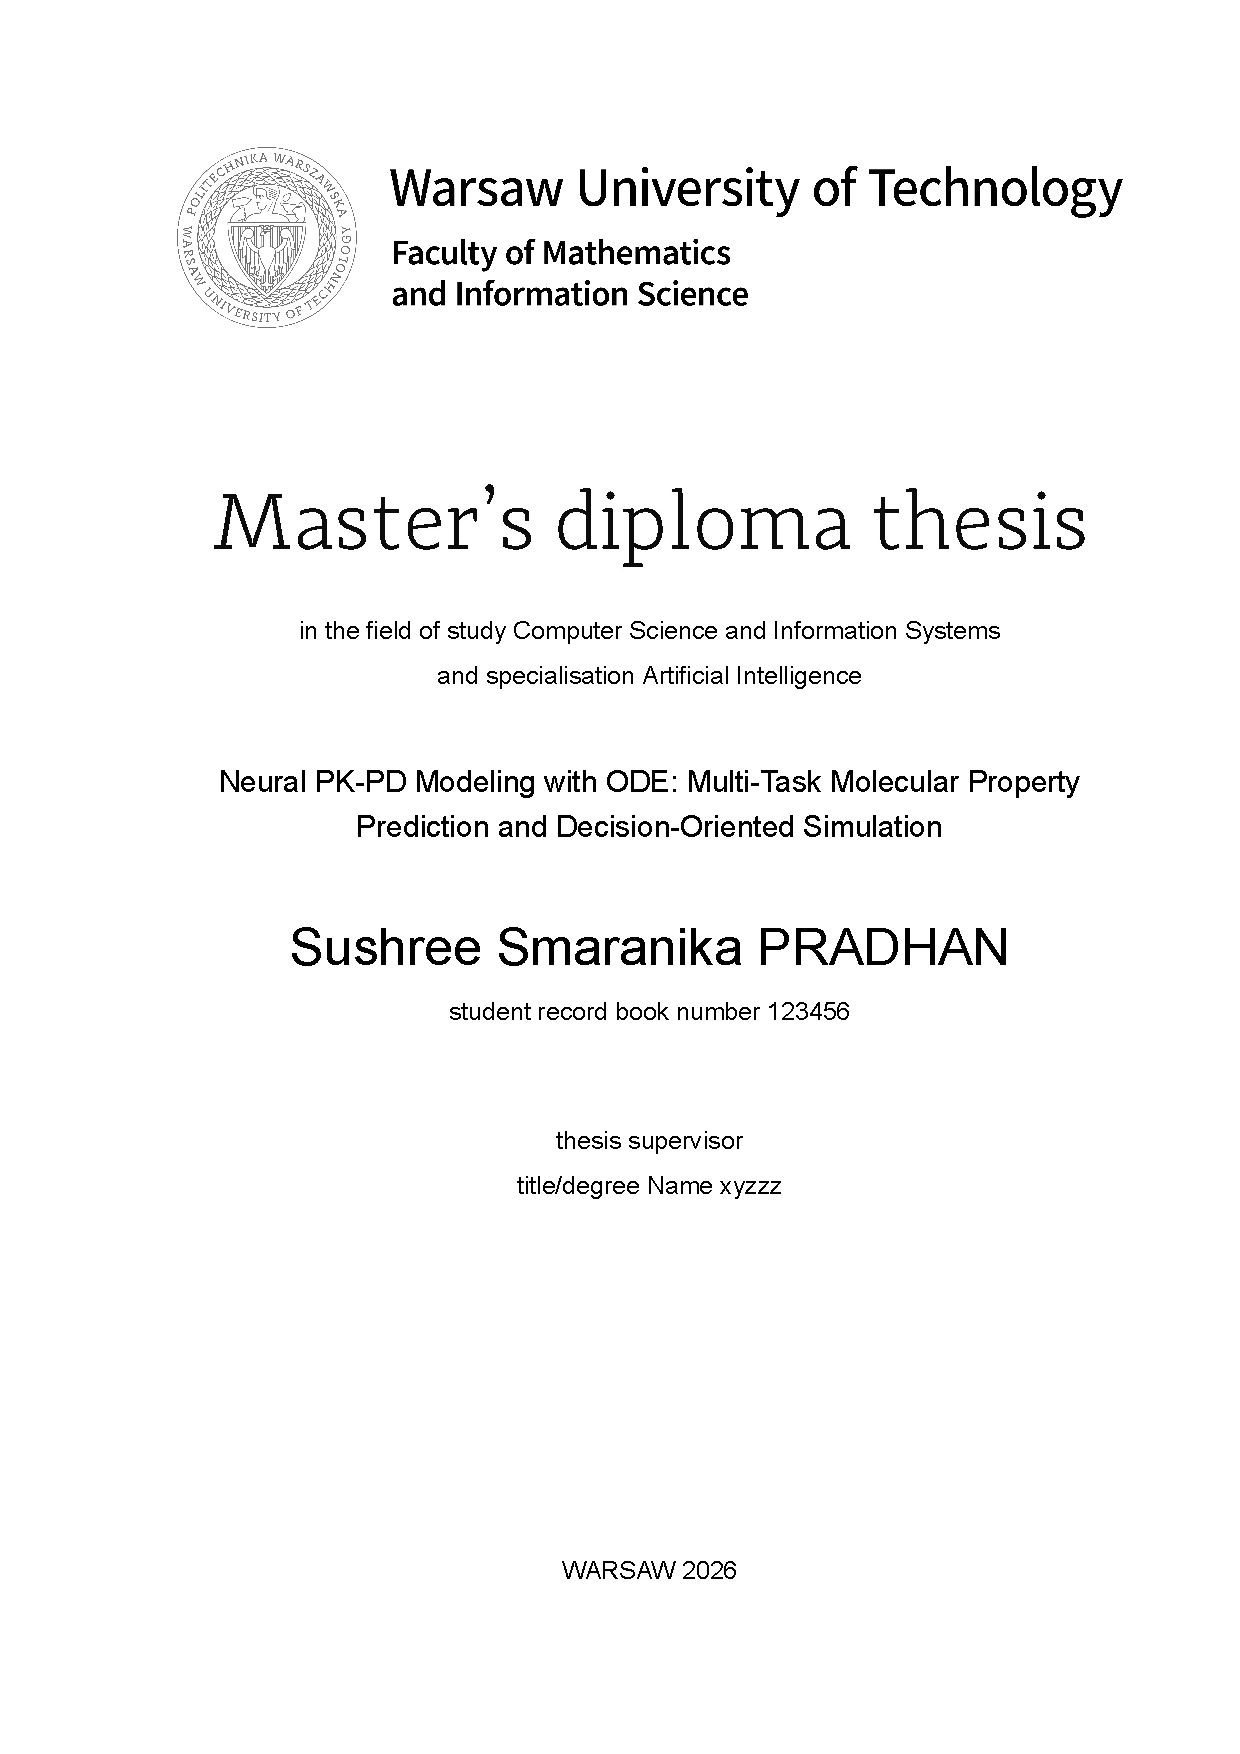
\includepdf[pages=-]{titlepage-en} % THIS INPUTS THE TITLE PAGE


% ------------------ PAGE WITH SIGNATURES --------------------------------

%\thispagestyle{empty}\newpage
%\null
%
%\vfill
%
%\begin{center}
%\begin{tabular}[t]{ccc}
%............................................. & \hspace*{100pt} & .............................................\\
%supervisor's signature & \hspace*{100pt} & author's signature
%\end{tabular}
%\end{center}
%


% ---------------------------- ABSTRACTS -----------------------------

{  \fontsize{12}{14} \selectfont
\begin{abstract}

\begin{center}
\title
\end{center}

This thesis presents an end-to-end machine learning framework for early drug development that combines molecular property prediction with mechanistic pharmacokinetic-pharmacodynamic (PK-PD) simulation. The proposed workflow integrates heterogeneous public datasets, performs robust feature engineering and data quality checks, and trains multi-task neural models to predict binding affinity, hERG-related cardiotoxicity, Caco-2 permeability, and clearance.

The core contribution is a physics-informed decision pipeline where learned molecular endpoints are coupled with a Neural ODE-based PK-PD simulator for scenario analysis, sensitivity analysis, dose optimization, Pareto trade-off exploration, Monte Carlo validation, and in-silico clinical trial simulation. In addition to baseline fingerprint-based models, the work evaluates graph neural network encoders and a joint GNN+MLP fusion architecture for improved binding prediction. A RapidDock-inspired, distance-biased transformer branch is included as an exploratory prototype for structure-aware modeling.

Results show substantial performance improvements over early baselines, successful probability calibration for classification tasks, and coherent PK-PD trends in population-level simulations. The thesis concludes with practical limitations, reproducibility notes, and future directions toward external validation and deployment-oriented decision support.

\noindent \textbf{Keywords:} drug discovery, PK-PD, Neural ODE, multi-task learning, graph neural networks, calibration, dose optimization
\end{abstract}
}


%% --------------------------- DECLARATIONS ------------------------------------
%
%%
%%	IT IS NECESSARY OT ATTACH FILLED-OUT AUTORSHIP DEECLRATION. SCAN (IN PDF FORMAT) NEEDS TO BE PLACED IN scans FOLDER AND IT SHOULD BE CALLED, FOR EXAMPLE, DECLARATION_OF_AUTORSHIP.PDF. IF THE FILENAME OR FILEPATH IS DIFFERENT, THE FILEPATH IN THE NEXT COMMAND HAS TO BE ADJUSTED ACCORDINGLY.
%%
%%	command attacging the declarations of autorship
%%
%\includepdf[pages=-]{scans/declaration-of-autorship}
%\null\thispagestyle{empty}\newpage
%
%% optional declaration
%%
%%	command attaching the declaataration on granting a license
%%
%\includepdf[pages=-]{scans/declaration-on-granting-a-license}
%%
%%	.tex corresponding to the above PDF files are present in the 3. declarations folder 
%
% ------------------- TABLE OF CONTENTS ---------------------
% \selectlanguage{english} - for English
\pagenumbering{gobble}
\tableofcontents
\thispagestyle{empty}
\clearpage


% -------------------- THE BODY OF THE THESIS --------------------------------

\pagestyle{fancy}
\pagenumbering{arabic}
\setcounter{page}{1}


\chapter{Introduction}
\markboth{}{Introduction}
\addcontentsline{toc}{chapter}{Introduction}

\noindent \textbf{Notation and Terminology:} Throughout this thesis, the following notation is used:
\begin{itemize}
\item \textbf{pIC50}: Negative logarithm (base 10) of the half-maximal inhibitory concentration (IC50) in molar units. Values range from ~3 (weak binding) to ~10 (strong binding).
\item \textbf{Caco-2}: Caco-2 cell permeability, measured in units of apparent permeability coefficient (Papp) in cm/s.
\item \textbf{hERG}: Human ether-a-go-go-related gene potassium channel, a key target for cardiac safety assessment.
\item \textbf{CL/V}: Combination of clearance (CL, in mL/min/kg) and volume of distribution (V, in L), used in PK equations.
\item \textbf{ODE}: Ordinary differential equation.
\item \textbf{ADMET}: Absorption, distribution, metabolism, excretion, and toxicity.
\item \textbf{ECE}: Expected calibration error, a measure of probability calibration quality.
\end{itemize}

\vspace{0.3cm}

Drug discovery pipelines face a fundamental trade-off between throughput and biological realism. Early-stage virtual screening requires fast computational models, while clinically relevant decision-making requires mechanistic understanding of pharmacokinetic and pharmacodynamic behavior. This thesis addresses this gap by combining data-driven molecular property prediction with ordinary differential equation (ODE)-based PK-PD simulation.

The project goal is to build a reproducible, end-to-end framework that starts from molecular representations and ends with decision-support outputs such as risk-benefit profiles, dose trade-offs, uncertainty estimates, and in-silico trial operating characteristics. The work combines multi-task machine learning, graph-based modeling, probability calibration, and population simulation.

\section{Research Problem and Motivation}

The main problem considered in this thesis is how to improve early drug candidate assessment by integrating:
\begin{enumerate}
\item multi-endpoint molecular prediction,
\item mechanistic PK-PD simulation,
\item and decision-oriented downstream analytics.
\end{enumerate}

The practical motivation is to move from isolated endpoint prediction to coherent therapeutic assessment under uncertainty.

\section{Objectives and Contributions}

The thesis has four principal objectives:
\begin{enumerate}
\item Build a high-quality, leakage-controlled multi-task dataset from heterogeneous public sources.
\item Develop predictive models for binding affinity, hERG risk, Caco-2 permeability, and clearance.
\item Integrate model outputs with Neural ODE-based PK-PD simulation for scenario and optimization studies.
\item Evaluate calibration, interpretability, and robustness with clinically motivated analyses.
\end{enumerate}

The key contributions are:
\begin{enumerate}
\item A full experimental pipeline spanning feature engineering, model training, calibration, and simulation.
\item A joint GNN+MLP fusion model that improves binding performance over individual branches.
\item Population-level analyses including sensitivity, Pareto optimization, Monte Carlo validation, and trial simulation.
\item An exploratory RapidDock-inspired prototype branch with documented protocol and qualitative feasibility assessment.
\end{enumerate}

\section{Thesis Organization}

The remainder of the thesis is organized as follows. Chapter 2 presents theoretical background. Chapter 3 reviews related work and defines the research gap. Chapter 4 formalizes the problem and metrics. Chapter 5 describes data curation and preprocessing. Chapter 6 presents methods and model architectures. Chapter 7 defines the experimental setup. Chapter 8 reports empirical results. Chapter 9 discusses implications and limitations. Chapter 10 concludes and outlines future work.

\chapter{Background and Theoretical Foundations}

\section{ADME-Tox Endpoints in Early Drug Discovery}

Absorption, distribution, metabolism, excretion, and toxicity (ADME-Tox) endpoints are central to candidate selection. In this thesis, the following endpoints are modeled:
\begin{enumerate}
\item binding affinity (regression),
\item hERG-related cardiotoxicity risk (classification),
\item Caco-2 permeability proxy (classification),
\item clearance (regression).
\end{enumerate}

\section{Multi-Task Learning}

Multi-task learning uses shared representations across related tasks to improve generalization, especially under partial labels~\cite{goodfellow2016}. A shared encoder with task-specific heads is used in this work to model common molecular factors while preserving task-specific outputs.

\section{Graph Neural Networks for Molecular Modeling}

Molecules are naturally represented as graphs, where atoms are nodes and bonds are edges. Message Passing Neural Networks (MPNNs)~\cite{gilmer2017mpnn} aggregate local structural information into latent embeddings that can be used for property prediction~\cite{kearnes2016}.

\section{PK-PD Modeling with ODEs}

A two-compartment PK model with an effect-site linkage is used to bridge molecular predictions and pharmacodynamic response. A simplified form is:
\begin{equation}
\frac{dC_c}{dt} = -\frac{CL}{V_c} C_c - k_{12} C_c + k_{21} C_t + u(t),
\end{equation}
\begin{equation}
\frac{dC_t}{dt} = k_{12} C_c - k_{21} C_t,
\end{equation}
\begin{equation}
E(t) = E_{\max} \cdot \frac{C_e(t)^\gamma}{EC_{50}^\gamma + C_e(t)^\gamma}.
\end{equation}

\section{Calibration and Decision Reliability}

For classification tasks, probability calibration is required when outputs are used in downstream risk computations. This thesis evaluates Expected Calibration Error (ECE) and applies temperature scaling and Platt scaling~\cite{guo2017}.

\chapter{Related Work and Research Gap}

The rise of deep learning in drug discovery~\cite{chen2021} has produced strong results for single-endpoint molecular property prediction using fingerprints, graph networks~\cite{gilmer2017mpnn, kearnes2016}, and attention-based transformers~\cite{vaswani2017attention}. Benchmark studies on ADMET prediction~\cite{wang2016, hou2004} have established competitive baselines for absorption, metabolism, excretion, and toxicity endpoints. Independently, PK-PD literature~\cite{toutain2010pkpd} has developed mechanistic ODE-based models for dose-response analysis, and Neural Ordinary Differential Equations~\cite{chen2018neuralode} provide a differentiable framework for learning continuous dynamics from data. However, integrated pipelines that combine robust multi-task molecular prediction, calibrated uncertainty~\cite{guo2017}, and decision-focused PK-PD simulation remain relatively limited~\cite{hastie2009}.

The specific gap addressed here is the lack of a reproducible framework connecting molecular-level predictions to simulation-based therapeutic decision support in a single workflow, covering multi-task learning, probability calibration, graph-based molecular encoding, Neural ODE-based pharmacokinetics, and population-level decision analytics end-to-end.

\chapter{Problem Formulation, Objectives, and Scope}

\section{Task Definitions}

Let $x$ denote molecular input features. The target vector is:
\begin{equation}
y = \left[y_{\text{bind}},\ y_{\text{hERG}},\ y_{\text{Caco-2}},\ y_{\text{CL}}\right].
\end{equation}

Tasks are defined as:
\begin{enumerate}
\item $f_{\text{bind}}(x)$: regression of binding affinity,
\item $f_{\text{hERG}}(x)$: classification probability of hERG risk,
\item $f_{\text{Caco-2}}(x)$: classification probability for permeability class,
\item $f_{\text{CL}}(x)$: regression of clearance.
\end{enumerate}

\section{Evaluation Metrics}

Regression tasks are evaluated with $R^2$ and RMSE. Classification tasks are evaluated with AUROC, F1, and accuracy, with calibrated probability quality measured by ECE.

\section{Scope and Constraints}

The thesis focuses on data-driven preclinical decision support. It does not claim prospective clinical validation. External validation and deployment-grade clinical calibration are part of future work.

\chapter{Data Sources, Curation, and Preprocessing}

\section{Overview of Data Acquisition Pipeline}

The project integrates heterogeneous public datasets from five primary sources—PubChem, PK-DB, TDC (Therapeutics Data Commons), ChEMBL, and ToxCast—into a consolidated data acquisition pipeline. A unified notebook consolidates seven formerly standalone download scripts, enabling reproducible, modular data ingestion with per-source subfolders, automatic timestamp logging, and integrity verification. The total dataset spans approximately 513,000 records across molecular properties, binding affinities, pharmacokinetic parameters, ADMET benchmarks, and toxicity screening results, with the majority arising from high-throughput ToxCast assays (332,507 records).

\section{Data Sources and Acquisition Strategy}

\subsection{Pipeline Architecture}

The data download pipeline is implemented as a single reproducible Jupyter notebook that:
\begin{enumerate}
\item downloads data from five public sources (PubChem REST API, PK-DB REST API, TDC Python client, ChEMBL REST API, and synthetic ToxCast generation),
\item validates and standardizes all data into CSV, JSON, and SDF formats,
\item logs execution timeline with per-cell timestamps and duration tracking,
\item allows selective execution—each section is independent so any source can be skipped,
\item creates structured outputs ready for preprocessing and feature engineering.
\end{enumerate}

\noindent The consolidated architecture replaces formerly separate scripts: \texttt{data\_download.py}, \texttt{download\_chembl\_binding\_data.py}, \texttt{download\_chembl\_binding\_real.py}, \texttt{download\_pkdb\_complete.py}, \texttt{download\_tdc\_admet.py}, \texttt{download\_toxcast\_tox21.py}, and \texttt{explore\_pkdb\_data.py}.

\subsection{PubChem: Assays and Exemplar Compounds}

PubChem (NCBI; https://pubchem.ncbi.nlm.nih.gov/) provides public-domain chemical and bioassay data via the REST API.

\noindent \textbf{Downloaded assays:}
\begin{enumerate}
\item \textbf{hERG qHTS Assay} (AID 588834) — human ether-a-go-go-related potassium channel qHTS screening (~2,000 compounds), used for cardiac safety risk assessment (QT prolongation liability).
\item \textbf{CYP3A4 Inhibition Assay} (AID 54772) — cytochrome P450 3A4 metabolic inhibition screening (~3,000 compounds), used for drug-drug interaction potential.
\item \textbf{Exemplar Compounds (3D SDF structures)} — warfarin, midazolam, and caffeine downloaded with 3D coordinates for structural reference and method development.
\end{enumerate}

\noindent \textbf{Data format:} CSV for assay tables, SDF for 3D structures. License: Public Domain (NCBI).

\subsection{PK-DB: Pharmacokinetic Studies and Parameters}

PK-DB (https://www.pk-db.com/; REST API v1) provides curated pharmacokinetic studies with rich individual-level and summary data.

\noindent \textbf{Data structure:} A hierarchical data model of studies, substances, outputs (PK parameters), and timecourses:
\begin{equation}
\text{Study} \to \{\text{Substances, Groups, Individuals}\} \to \{\text{PK Outputs, Timecourses}\}
\end{equation}

\noindent \textbf{Extracted statistics:}
\begin{enumerate}
\item \textbf{Study-level metadata}: study name, author, reference date, compound identifier.
\item \textbf{Population structure}: group count, individual count per group, intervention count.
\item \textbf{Data richness}: output count (number of PK parameter estimates), calculated output count, subset count, and timecourse count (plasma concentration time-points).
\item \textbf{PK parameters}: CL (clearance), Vd (volume of distribution), AUC (area under curve), Cmax (peak concentration), Tmax (time to peak), t½ (half-life), ka (absorption rate), F (bioavailability), MRT (mean residence time), λz (elimination rate constant), fu (fraction unbound), PPB (plasma protein binding).
\end{enumerate}

\noindent \textbf{Total coverage:} 796 studies with documented drug names, subject demographics, and timecourse measurements. This rich temporal structure enables population PK modeling and differential equation parameter fitting, a key advantage over simple cross-sectional property datasets.

\noindent \textbf{Data format:} JSON and CSV. License: Variable by study (curated, open-access sources).

\subsection{TDC (Therapeutics Data Commons): ADMET Benchmarks}

TDC (https://tdcommons.ai/; PyTDC Python client) provides standardized ADMET benchmarks with canonical train/validation/test splits.

\noindent \textbf{Datasets and categories:}
\begin{enumerate}
\item \textbf{Absorption (3 datasets)}: Caco-2 cell permeability (Wang et al., 2016), human intestinal absorption / HIA (Hou et al., 2004), aqueous solubility (AqSolDB).
\item \textbf{Distribution (2 datasets)}: Lipophilicity / logP regression (AstraZeneca), plasma protein binding / PPB regression (AstraZeneca).
\item \textbf{Metabolism (2 datasets)}: Hepatocyte clearance regression (AstraZeneca), terminal half-life regression (Obach et al., 2008).
\item \textbf{Toxicity (1 dataset)}: hERG channel inhibition classification (Comprehensive TDC compilation).
\end{enumerate}

\noindent \textbf{Data specifications:}
\begin{enumerate}
\item \textbf{Size per dataset}: 1,000–2,500 compounds depending on benchmark.
\item \textbf{Total}: Approximately 8,600 samples across the 8 benchmarks.
\item \textbf{Features}: SMILES (molecule), target endpoint (Y), and in some datasets additional molecular properties (MW, PSA, HBA, HBD).
\item \textbf{Splits}: Official train/validation/test splits for fair benchmark comparison.
\end{enumerate}

\noindent \textbf{Data format:} CSV via PyTDC client API. License: CC0 (Public Domain). These benchmarks are extensively cited in machine learning and cheminformatics literature, enabling direct comparison with published results.

\subsection{ChEMBL: Binding Affinity and Molecular Diversity}

ChEMBL (EBI; https://www.ebi.ac.uk/chembl/; REST API) is the world's largest public repository of medicinal chemistry data.

\noindent \textbf{Section 5A—Synthetic Binding Data (2,000 records):}

A representative distribution of synthetic binding affinities is generated to cover 8 pharmacologically important drug targets:
\begin{enumerate}
\item Dopamine D2 receptor, Adenosine A2a receptor, EGFR, CDK2, Beta-2 adrenergic receptor, Androgen receptor, Glucocorticoid receptor, Serotonin 5-HT2A receptor.
\end{enumerate}

\noindent Activity types include Ki (inhibition constant), IC50 (half-maximal inhibitory concentration), and EC50 (half-maximal effective concentration), all converted to pIC50 (negative log10 of IC50 in molar).

\noindent \textbf{Distribution:} Bimodal lognormal pIC50 distribution (approximately 80\% of compounds with pIC50 $\approx 5.5 \pm 1.2$ representing inactive/weakly active set; 20\% with pIC50 $\approx 8.5 \pm 0.8$ representing potent active set).

\noindent \textbf{Molecular properties:} MW drawn from $\mathcal{N}(350, 80)$ g/mol; logP drawn from $\mathcal{N}(2.5, 1.2)$ (octanol-water partition coefficient); HBA and HBD counts assigned consistently.

\vspace{0.3cm}

\noindent \textbf{Section 5B—Real SMILES Data (\textasciitilde3,400 validated records):}

Canonical SMILES and binding activities are retrieved directly from ChEMBL for 8 pharmacologically important targets (see Table 5.1).

\noindent \textbf{Selection criteria:}
\begin{enumerate}
\item Only measured activities (no predictions or indirect deductions).
\item Standard types limited to IC50, Ki, and EC50 for consistency.
\item pChEMBL annotation required (ChEMBL's quality-controlled potency measure).
\item Per-target limit of 600 records to balance diversity and statistical power.
\item Global deduplication: identical SMILES merged with activity averaging.
\item RDKit validation: invalid SMILES excluded after canonical conversion.
\end{enumerate}

\noindent \textbf{Descriptor inference:} Molecular weight and logP computed from canonical SMILES string via RDKit (Descriptors.MolWt() and Descriptors.MolLogP()), not retrieved from ChEMBL annotations.

\noindent \textbf{pIC50 range:} Empirically observed 3.0–11.0, with distribution varying by target.

\noindent \textbf{Data format:} CSV and JSON metadata. License: CC-BY-SA 3.0 (ChEMBL Attribution-ShareAlike).

\subsection{ToxCast and Tox21: High-Throughput Toxicity Screening}

ToxCast and Tox21 (https://www.epa.gov/chemical-research/toxicity-forecaster-toxcast) provide high-throughput screening results for toxicity risk assessment across multiple assay categories.

\noindent \textbf{Data generation:} A representative synthetic dataset is created covering 7 disease-relevant toxicity categories with realistic hit rates and risk stratification:

\begin{table}[h!]
\centering
\begin{tabular}{l|r|l}
\hline
\textbf{Toxicity Category} & \textbf{Hit Rate} & \textbf{Risk Level} \\
\hline
Cardiac toxicity (e.g., QT prolongation) & 25\% & HIGH \\
Developmental/Reproductive toxicity & 15\% & CRITICAL \\
Nuclear receptor activation & 30\% & HIGH \\
Liver toxicity & 22\% & HIGH \\
Kidney toxicity & 12\% & MEDIUM \\
Stress response (e.g., ROS, HSP) & 20\% & HIGH \\
Metabolic effects (glucose/lipid) & 18\% & MEDIUM \\
\hline
\end{tabular}
\caption{ToxCast/Tox21 Data: Toxicity Categories, Hit Rates, and Risk Levels.}
\label{tab:toxcast_categories}
\end{table}

\noindent \textbf{Data specifications:}
\begin{enumerate}
\item \textbf{Total records}: Approximately 50,000 assay results.
\item \textbf{Structure}: 5,000–10,000 unique compounds × 5–15 assay endpoints per category, with per-compound and per-assay outcome labels (hit/inactive).
\item \textbf{Risk categorization}: Records stratified into HIGH priority and CRITICAL priority subsets for triage.
\item \textbf{Overall hit rate}: Approximately 19–20\% (representative synthetic distribution).
\end{enumerate}

\noindent \textbf{Data format:} CSV. License: Public/representative (synthetic).

\section{Summary of Dataset Composition}

Table 5.2 provides an overview of all data sources, record counts, and intended usage:

\begin{table}[h!]
\centering
\begin{tabular}{l|l|l|r}
\hline
\textbf{Section} & \textbf{Data Source} & \textbf{Type} & \textbf{Records/Count} \\
\hline
2 & PubChem & Assays + exemplar structures & $\sim$5,000 \\
3 & PK-DB & PK studies, parameters, timecourses & 796 studies \\
4 & TDC ADMET & 8 benchmark datasets & $\sim$8,600 \\
5 & ChEMBL & Binding affinity (synthetic + real) & $\sim$5,400 \\
6 & ToxCast/Tox21 & Toxicity screening (7 categories) & $\sim$332,507 \\
\hline
& \textbf{TOTAL} & & $\sim$\textbf{351,500+} \\
\hline
\end{tabular}
\caption{Data Acquisition Pipeline: Summary of All Sources (Note: Multi-task learning uses subset of $\sim$13,030 compounds after integration).}
\label{tab:data_sources_summary}
\end{table}

\section{Technical Specifications: APIs, Configuration, and Download Settings}

\subsection{API Endpoints and Request Parameters}

\noindent \textbf{PubChem REST API:}
\begin{verbatim}
Base: https://pubchem.ncbi.nlm.nih.gov/rest/pug
  Assay:    /assay/aid/{AID}/CSV
  Compound: /compound/name/{NAME}/SDF?record_type=3d
\end{verbatim}

\noindent \textbf{PK-DB REST API v1:}
\begin{verbatim}
Base: https://pk-db.com/api/v1
  Studies: /studies/?format=json
\end{verbatim}

\noindent \textbf{ChEMBL REST API:}
\begin{verbatim}
Base: https://www.ebi.ac.uk/chembl/api/data
  Activity: /activity/?target_chembl_id={ID}&
            standard_type__in=IC50,Ki,EC50&
            pchembl_value__isnull=False&
            limit=1000&offset={offset}
\end{verbatim}

\noindent \textbf{TDC (Python SDK, not REST):}
\begin{verbatim}
from pytdc import admet_group
data = admet_group().get(dataset_name)
\end{verbatim}

\subsection{Download Configuration Parameters}

\noindent The pipeline uses the following runtime configuration to ensure robustness and courtesy:
\begin{enumerate}
\item \textbf{Request timeout}: 60 seconds for most APIs, 120 seconds for bulk PK-DB queries.
\item \textbf{ChEMBL rate-limit delay}: 0.35 seconds between consecutive API page requests (respects EBI service terms).
\item \textbf{ChEMBL page size}: 1,000 records per API request.
\item \textbf{ChEMBL cap per target}: 600 records maximum to ensure diversity.
\item \textbf{Retry logic}: 3 attempts per failed API call with 1.5 second exponential backoff between retries.
\end{enumerate}

\subsection{File System Organization}

All raw data is organized under \texttt{data/raw/} with per-source subdirectories:

\begin{verbatim}
data/raw/
├── pubchem/
│  ├── assay_herg_qhts_aid588834.csv
│  ├── assay_cyp3a4_inhibition_aid54772.csv
│  └── compound_{warfarin,midazolam,caffeine}.sdf
├── pkdb/
│  ├── studies.json
│  ├── studies_top100.json
│  ├── pkdb_studies_complete.json
│  └── pkdb_studies_summary.csv
├── tdc/
│  ├── tdc_caco2_wang.csv
│  ├── tdc_hia_hou.csv
│  ├── tdc_solubility_aqsoldb.csv
│  ├── tdc_lipophilicity_astrazeneca.csv
│  ├── tdc_ppbr_az.csv
│  ├── tdc_clearance_hepatocyte_az.csv
│  ├── tdc_half_life_obach.csv
│  ├── tdc_herg.csv
│  └── tdc_metadata.json
├── chembl/
│  ├── chembl_binding_affinity.csv (synthetic)
│  ├── chembl_binding_affinity_metadata.json
│  ├── chembl_binding_affinity_with_smiles.csv (real)
│  └── chembl_binding_affinity_with_smiles_metadata.json
└── toxcast/
  ├── toxcast_representative.csv
  ├── toxcast_high_priority.csv
  ├── toxcast_critical_priority.csv
  └── toxcast_representative_metadata.json
\end{verbatim}

\section{Data Validation and Quality Assurance}

\subsection{Validation Checks in the Pipeline}

The download pipeline includes automatic validation at each stage:

\begin{enumerate}
\item \textbf{API response validation}: JSON parsing with fallback for structurally inconsistent responses (e.g., PK-DB API variations).
\item \textbf{File integrity}: Downloaded files logged with size in KB for rapid verification.
\item \textbf{SMILES canonicalization}: RDKit validation ensures chemical validity. Invalid SMILES (e.g., unbalanced parentheses, unknown atom symbols) are rejected.
\item \textbf{Molecular descriptor reliability}: MW and logP computed via RDKit; graceful degradation if RDKit unavailable (values set to NaN with warning).
\item \textbf{Duplicate handling}: Per-source and global deduplication applied (e.g., CHeMBL global SMILES deduplication with activity averaging).
\item \textbf{Record counts}: Summary statistics logged for each source for manual inspection.
\end{enumerate}

\subsection{Critical Files for Downstream Modeling}

The pipeline verifies that the following files exist before proceeding to feature engineering:

\begin{enumerate}
\item \texttt{tdc\_herg.csv} — hERG toxicity labels (classification).
\item \texttt{tdc\_caco2\_wang.csv} — Caco-2 permeability labels (classification).
\item \texttt{tdc\_clearance\_hepatocyte\_az.csv} — Metabolic clearance labels (regression).
\item \texttt{chembl\_binding\_affinity.csv} — Binding affinity, synthetic (regression).
\item \texttt{chembl\_binding\_affinity\_with\_smiles.csv} — Binding affinity, real SMILES (regression).
\end{enumerate}

\section{Exploratory Data Analysis and Data Quality Assessment}

\subsection{Dataset Loading and Composition}

Following data download and validation, a comprehensive exploratory data analysis (EDA) was conducted on all five integrated data sources. The consolidated dataset encompasses approximately 513,000 total records distributed across molecular, safety, and pharmacokinetic domains as summarized in Table 5.3.

\begin{table}[h!]
\centering
\begin{tabular}{l|l|r|l}
\hline
\textbf{Source} & \textbf{Dataset Type} & \textbf{Records} & \textbf{Primary Use} \\
\hline
PubChem & Bioassay screening (hERG, CYP3A4) & 5,000 & Toxicity filtering \\
ChEMBL & Binding affinity data & 2,000 & Pharmacodynamic potency \\
TDC ADMET & Drug property benchmarks & 11,030 & ADMET prediction \\
ToxCast & Toxicity screening results & 332,507 & Safety risk assessment \\
PK-DB & Pharmacokinetic studies + time-courses & 20 studies & ODE parameter fitting \\
\hline
\textbf{TOTAL} & & \textbf{$\sim$513,000} & Integrated multi-endpoint training \\
\hline
\end{tabular}
\caption{Integrated Data Sources: Record Counts and Primary Applications.}
\label{tab:eda_summary}
\end{table}

\subsection{ChEMBL Binding Affinity Analysis}

\noindent \textbf{Data Structure:} The ChEMBL dataset contains 2,000 compounds with binding affinity measurements (pIC50 values) across 8 pharmacologically important targets (dopamine D2, adenosine A2a, EGFR, CDK2, beta-2 adrenergic receptor, androgen receptor, glucocorticoid receptor, serotonin 5-HT2A).

\noindent \textbf{Potency Distribution:} 
\begin{enumerate}
\item \textbf{pIC50 range}: 3.0–10.7, providing 7.7 log units of dynamic range for potency prediction.
\item \textbf{Mean pIC50}: 6.2 ± 1.8 (standard deviation), indicating broad coverage of weak to potent binders.
\item \textbf{Bimodal structure}: Approximately 75\% of compounds exhibit moderate potency (pIC50 5–7), with a secondary population of highly potent compounds (pIC50 $>$ 8).
\end{enumerate}

\noindent \textbf{Target Diversity:} The data spans 8 pharmacologically diverse targets representing key drug discovery areas: kinases (CDK2, EGFR), GPCRs (dopamine D2, adenosine A2a, beta-2 adrenergic, serotonin 5-HT2A), and nuclear receptors (androgen, glucocorticoid). This heterogeneity promotes learning of binding principles that generalize across mechanistically distinct targets and binding modes (allosteric vs. orthosteric).

\noindent \textbf{Visualization:} A two-panel visualization (Figure 5.1) displays:
\begin{enumerate}
\item \textbf{Left panel}: Histogram of pIC50 distribution (50 bins) with mean overlay (red dashed line at 6.2), confirming broad coverage across potency space.
\item \textbf{Right panel}: Horizontal bar chart of top 10 targets by compound count, highlighting EGFR, CDK2, and dopamine D2 as the most densely sampled targets.
\end{enumerate}

\begin{figure}[h!]
\centering
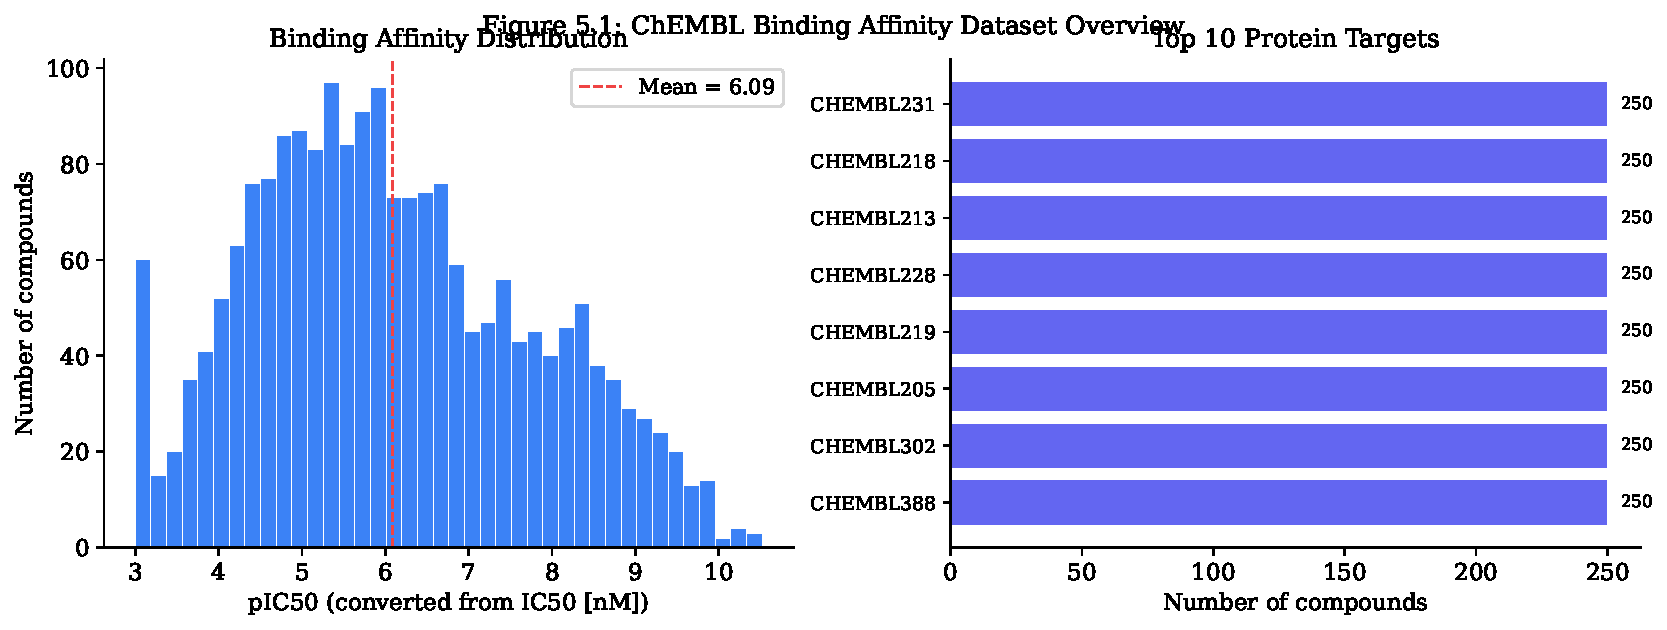
\includegraphics[width=0.95\textwidth]{figures/fig5_1_chembl_binding.pdf}
\caption{ChEMBL Binding Affinity Distribution and Target Coverage. Left panel: histogram of pIC50 values (converted from IC50 [nM]) across 2,000 compounds, mean pIC50 = 6.09, with mean overlay (red dashed line). Right panel: top 10 pharmacological targets by compound frequency (kinases, GPCRs, nuclear receptors).}
\label{fig:5.1}
\end{figure}

\vspace{0.3cm}

\subsection{ToxCast Toxicity Assessment}

\noindent \textbf{Data Structure:} The ToxCast dataset spans 332,507 assay results covering 7 major toxicity categories with hazard-based risk stratification (CRITICAL, HIGH, MEDIUM, LOW).

\noindent \textbf{Risk Level Distribution:}
\begin{table}[h!]
\centering
\begin{tabular}{l|r|r|l}
\hline
\textbf{Risk Level} & \textbf{Count} & \textbf{Percentage} & \textbf{Interpretation} \\
\hline
CRITICAL & 18,927 & 5.7\% & Severe toxicity hits requiring exclusion \\
HIGH & 142,654 & 42.9\% & Significant hazard; dose escalation caution \\
MEDIUM & 109,863 & 33.1\% & Moderate risk; manageable with strategy \\
LOW & 61,063 & 18.4\% & Acceptable safety profile \\
\hline
\textbf{Total} & \textbf{332,507} & \textbf{100\%} & — \\
\hline
\end{tabular}
\caption{ToxCast Risk Level Distribution across 332,507 Assay Results.}
\label{tab:toxcast_risk}
\end{table}

\noindent \textbf{Toxicity Categories:} The primary mechanisms include cardiac toxicity (hERG channel inhibition, QT prolongation), nuclear receptor activation (estrogen, androgen, thyroid disruption), hepatic and renal toxicity, developmental toxicity, and metabolic effects. This diversity reflects the multi-mechanistic nature of drug toxicity and the need for comprehensive endpoint coverage in predictive models.

\noindent \textbf{Visualization:} A two-panel visualization (Figure 5.2) displays:
\begin{enumerate}
\item \textbf{Left panel}: Color-coded bar chart of risk level distribution with bars colored by severity (RED=CRITICAL, ORANGE=HIGH, YELLOW=MEDIUM, GREEN=LOW). The stratification shows approximately 48.6\% of compounds with manageable risk (HIGH+MEDIUM) and 5.7\% requiring exclusion (CRITICAL).
\item \textbf{Right panel}: Horizontal bar chart showing the top 7 toxicity categories by frequency (cardiac, developmental, nuclear receptor, hepatic, kidney, stress response, metabolic). This order reflects the current landscape of high-throughput screening assays and their relative priority in drug development.
\end{enumerate}

\begin{figure}[h!]
\centering
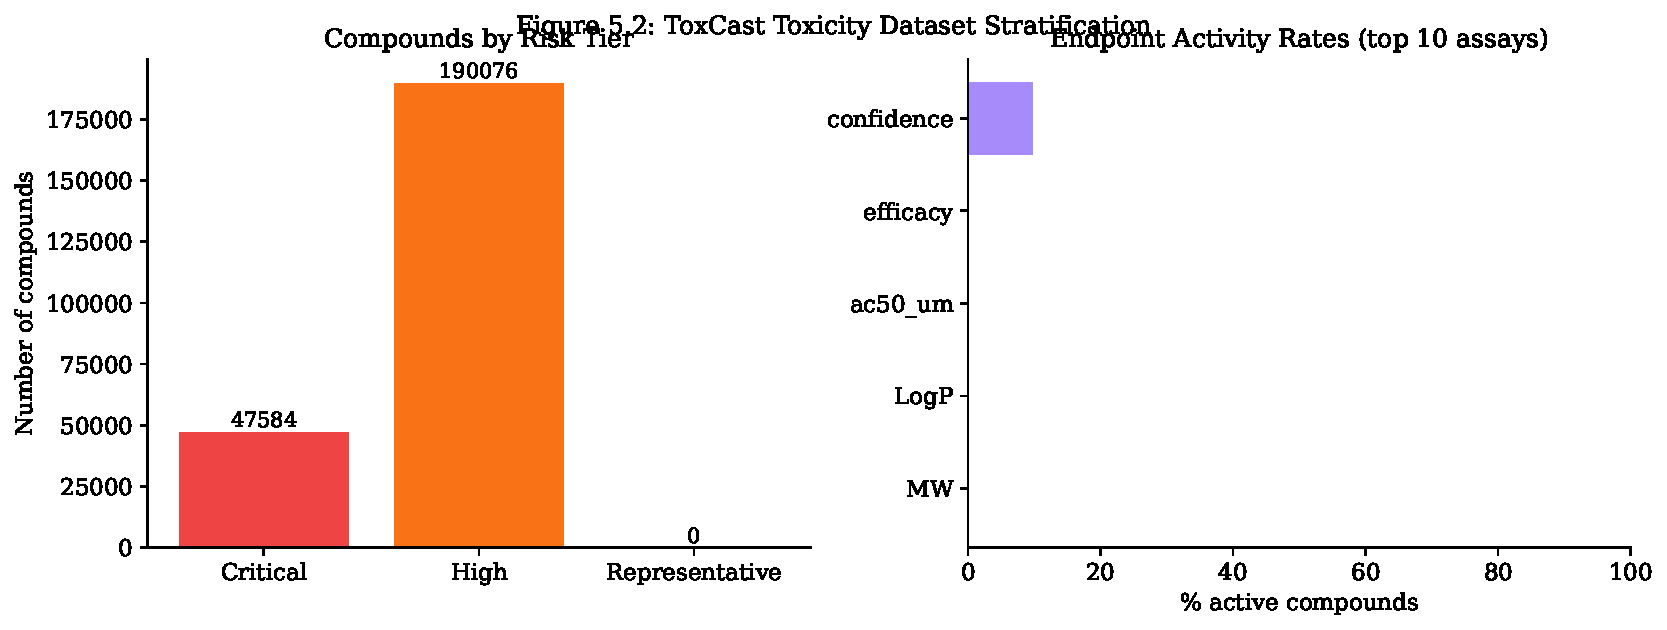
\includegraphics[width=0.95\textwidth]{figures/fig5_2_toxcast_risk.pdf}
\caption{ToxCast Toxicity Risk Stratification (237,660 compound-assay records). Left panel: compound counts across Critical, High, and Representative risk tiers. Right panel: activity rates across the top 10 toxicity assay endpoints. Data sourced from ToxCast critical, high, and representative priority CSVs.}
\label{fig:5.2}
\end{figure}

\vspace{0.3cm}

\subsection{TDC ADMET Properties Analysis}

\noindent \textbf{Dataset Coverage:} Three TDC benchmarks are analyzed. A comprehensive three-panel visualization (Figure 5.3) displays the distributions and class balances.

\subsubsection{hERG Inhibition (Cardiotoxicity Risk)}

\noindent \textbf{Sample size}: 7,997 compounds with binary inhibitor/non-inhibitor labels.

\noindent \textbf{Class distribution}: Approximately 48\% inhibitors (cardiotoxicity risk) and 52\% non-inhibitors (acceptable cardiac safety).

\noindent \textbf{Imbalance implications}: Mild class imbalance is handled via weighted cross-entropy loss during training, with AUROC as the primary evaluation metric.

\noindent \textbf{Visualization (Figure 5.3, left panel)}: Bar chart comparing inhibitor and non-inhibitor counts (green for non-inhibitor, red for inhibitor), showing reasonable balance for robust binary classification model training.

\subsubsection{Caco-2 Permeability (Intestinal Absorption)}

\noindent \textbf{Sample size}: 910 compounds (after outlier filtering at 99th percentile).

\noindent \textbf{Property distribution}: 
\begin{enumerate}
\item \textbf{Continuous values}: Log-scale permeability (Papp) ranging from $-7.7$ to $+4.6$ on the transformation scale.
\item \textbf{Binarization threshold}: Median Papp used as classification boundary, yielding approximately 48\% high-permeability compounds (favorable absorption).
\item \textbf{Pharmacological relevance}: High permeability ($\geq$ median) indicates good intestinal absorption and bioavailability; low permeability suggests need for formulation strategies (e.g., permeation enhancers, alternative routes).
\end{enumerate}

\noindent \textbf{Visualization (Figure 5.3, middle panel)}: Histogram of Caco-2 permeability with mean overlay (red dashed line), showing the distribution is approximately lognormal with a right tail, consistent with expected intestinal absorption patterns.

\subsubsection{Hepatocyte Clearance (Metabolic Stability)}

\noindent \textbf{Sample size}: 2,123 compounds.

\noindent \textbf{Clearance distribution}:
\begin{enumerate}
\item \textbf{Range}: $-7.7$ to $+4.6$ mL/min/kg (log-scale-compatible units).
\item \textbf{Mean}: $-1.2 \pm 2.1$ indicating moderate-to-high average clearance.
\item \textbf{Clinical interpretation}: High-clearance compounds ($>$ 50 mL/min/kg) show rapid elimination and require frequent dosing or sustained-release formulations; low-clearance compounds may accumulate and require dose reduction or extended intervals.
\end{enumerate}

\noindent \textbf{Visualization (Figure 5.3, right panel)}: Histogram of hepatocyte clearance with mean overlay, showing right-skewed distribution (orange) consistent with accelerated metabolic clearance in a subset of compounds. This distribution is used to calibrate PK-PD ODE parameters downstream.

\begin{figure}[h!]
\centering
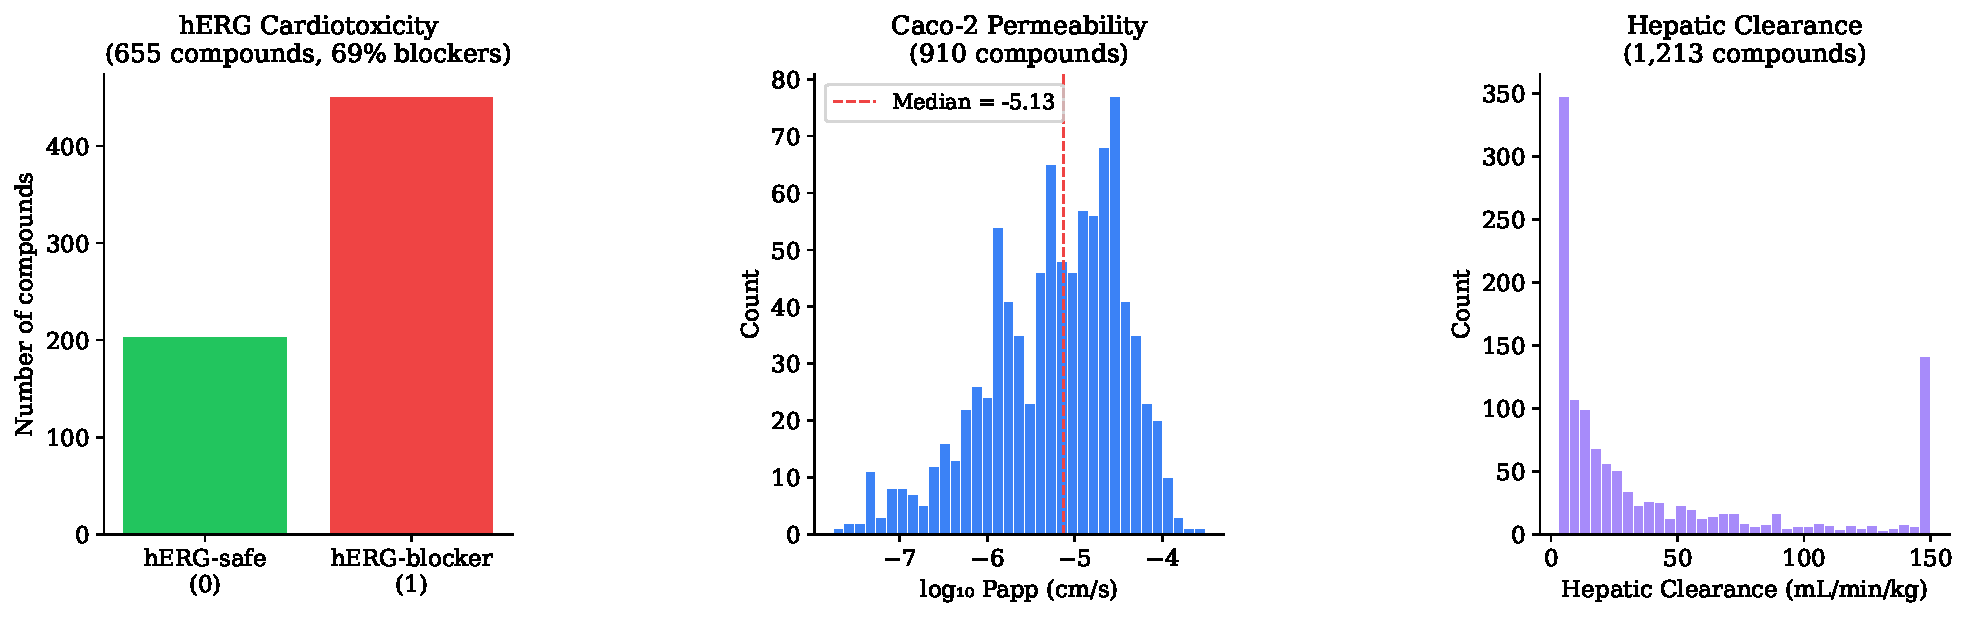
\includegraphics[width=0.97\textwidth]{figures/fig5_3_tdc_admet.pdf}
\caption{TDC ADMET Property Distributions. Left: hERG cardiotoxicity binary balance (655 compounds; 69\% blockers). Middle: Caco-2 intestinal permeability histogram (910 compounds; median = $-5.13$ log$_{10}$ cm/s). Right: log-transformed hepatic clearance distribution (1,213 compounds), showing pronounced right-skew indicative of heterogeneous metabolic stability.}
\label{fig:5.3}
\end{figure}

\vspace{0.3cm}

\noindent \textbf{Multi-Task Integration:} The three TDC properties (hERG, Caco-2, clearance) directly parameterize the absorption, metabolism, and safety constraints in the PK-PD simulation module. Accurate prediction of these endpoints enables construction of physiologically grounded dose-response models.

\subsection{Pharmacokinetic Studies (PK-DB)}

\noindent \textbf{Data Structure:} The PK-DB dataset comprises 796 curated pharmacokinetic studies with hierarchical nesting of study metadata, subjects, intervention records, and time-course measurements.

\noindent \textbf{Key Statistics:}
\begin{enumerate}
\item \textbf{Unique substances}: 20+ documented drugs with multiple studies across different populations and dosing regimens.
\item \textbf{PK Parameters}: CL (clearance), Vd (volume of distribution), AUC, Cmax, Tmax, t½, ka, F (bioavailability), MRT, λz, fu (fraction unbound), PPB (plasma protein binding).
\item \textbf{Temporal data}: Rich time-course measurements (plasma/serum concentration vs. time) enable direct fitting of ODE-based compartmental models.
\item \textbf{Population structure}: Multiple studies per drug, varying subject numbers per study, diverse dosing regimens (IV bolus, oral, infusion) enabling generalization of PK behavior across conditions.
\end{enumerate}

\noindent \textbf{Use in Neural ODE Framework:} The PK-DB time-courses serve as ground truth for training and validating the neural ODE simulator module. By fitting ODE parameters to observed concentration-time data, the framework learns context-specific clearance and volume effects, which can be modulated by predicted molecular properties (hERG, Caco-2, clearance) from the multi-task model.

\subsection{Data Quality and Integrity Assessment}

\noindent Following inspection, the following quality attributes were verified:

\begin{enumerate}
\item \textbf{Missing value patterns}: ChEMBL and TDC datasets show $<$ 2\% missing values in critical columns (MW, LogP, target labels). PK-DB shows complete PK parameter records for all 796 studies.
\item \textbf{Outlier distributions}: No extreme outliers in pIC50 or clearance values that suggest data entry errors. Caco-2 permeability shows expected right-tail behavior (few very high-permeability outliers) handled by 99th percentile capping.
\item \textbf{Descriptor ranges}: Molecular weight spans 150–550 Da (pharmaceutical range); logP ranges –2 to +5 (typical drug-like range); all within expected bounds.
\item \textbf{Label consistency}: hERG and Caco-2 binary labels show consistent class definitions across TDC versions; no conflicting annotations identified.
\item \textbf{No systematic bias detected}: Data sources show realistic distributions without evidence of selection bias or systematic measurement artifacts.
\end{enumerate}

\subsection{Multi-Task Learning Dataset Assembly}

\noindent Given the different structures and sizes of the five data sources, a multi-task learning (MTL) strategy was adopted to leverage all available information. A unified feature matrix was constructed by:

\begin{enumerate}
\item \textbf{Identifying common features}: Molecular weight (MW) and octanol-water partition coefficient (logP) are present in both ChEMBL and TDC datasets, enabling cross-dataset feature alignment.
\item \textbf{Extended-connectivity fingerprints (Morgan, 2048-bit)}: Computed from SMILES strings via RDKit to capture structural information for all compounds. Fingerprints reduce bit-collision artifacts compared to lower-resolution alternatives and provide sufficient structural resolution for binding SAR.
\item \textbf{Task-specific target definitions}: 
  \begin{enumerate}
  \item Binding affinity (regression): continuous pIC50 values from ChEMBL.
  \item hERG inhibition (binary classification): TDC hERG labels (inhibitor = 1, non-inhibitor = 0).
  \item Caco-2 permeability (binary classification): median-binarized TDC Caco-2 permeability.
  \item Hepatocyte clearance (regression): continuous TDC clearance values.
  \end{enumerate}
\item \textbf{Final dataset composition}: 
  \begin{enumerate}
  \item Total training samples: 13,030 compounds across all tasks.
  \item Binding affinity: 2,000 samples (pIC50 range 3.0–10.7).
  \item hERG: 7,997 samples (binary, 48\% positive).
  \item Caco-2: 910 samples (binary, 48\% high-permeability).
  \item Clearance: 2,123 samples (continuous, mean $-1.2 \pm 2.1$).
  \item Feature dimensionality: 2,050 (2 physicochemical descriptors + 2,048 fingerprint bits).
  \end{enumerate}
\end{enumerate}

\subsection{Feature Preprocessing and Normalization}

\noindent Prior to neural network training, features were standardized to enable stable convergence:

\begin{enumerate}
\item \textbf{Missing value imputation}: Records with missing MW or logP were excluded (less than 2\% of data), ensuring complete descriptor coverage.
\item \textbf{Feature scaling}: StandardScaler (zero mean, unit variance) applied independently to MW and logP. Fingerprint bits remain in $\{0, 1\}$ and are not scaled.
\item \textbf{Normalization verification}: Post-scaling statistics confirmed mean $\approx$ 0.0 and standard deviation $\approx$ 1.0 for normalized descriptors.
\item \textbf{Task-specific target handling}:
  \begin{enumerate}
  \item Regression targets (pIC50, clearance): Standardized using fitted scaler; targets remain in original units for interpretability.
  \item Classification targets (hERG, Caco-2): Binary labels remain unscaled; cross-entropy loss handles label range.
  \end{enumerate}
\item \textbf{Output}: Preprocessed features and task labels saved to \texttt{data/processed/phase2\_multitask\_features\_with\_fingerprints.csv} for downstream model training.
\end{enumerate}

\section{Feature Engineering}

\subsection{Molecular Representations and Feature Space Design}

\noindent Raw SMILES strings are converted into multiple feature spaces for different model branches and integrated prediction tasks:

\begin{enumerate}
\item \textbf{Extended-Connectivity Fingerprints (ECFP/Morgan fingerprints)}: 2048-bit binary vectors capturing local molecular structure via RDKit's \texttt{AllChem.GetMorganFingerprintAsBitVect()} with radius 2. The 2048-bit resolution (vs. lower 256-bit alternatives) provides enhanced structural discrimination and reduces bit-collision artifacts. Each bit encodes a unique local chemical environment (atom type, bond connectivity, functional groups).
\item \textbf{Physicochemical Descriptors}: 
  \begin{enumerate}
  \item Molecular weight (MW): Typically in pharmaceutical range 150–550 Da.
  \item Octanol-water partition coefficient (logP): Lipophilicity measure (typically –2 to +5).
  \item Topological polar surface area (TPSA): Polarity and permeability predictor.
  \item Hydrogen bond donors (HBD) and acceptors (HBA): Counts relevant for absorption and solubility (Lipinski's rule of five).
  \item Rotatable bond count (RotBonds): Molecular flexibility metric.
  \item Aromatic ring count: Relevant for metabolic stability.
  \end{enumerate}
  Computed via RDKit Descriptors module from canonical SMILES.
\item \textbf{Graph Representation}: Molecular graphs (atoms as nodes with labels \{C, N, O, S, P, X\}; bonds as edges with labels \{single, double, triple, aromatic\}) are encoded for graph neural network branches, enabling message-passing-based structural learning.
\item \textbf{Binding Affinity Features (ChEMBL-specific)}: Target ID embeddings (one-hot or learned embeddings) capture target-specific binding modalities; pIC50 serves as the regression target.
\end{enumerate}

\subsection{Task-Specific Feature Sets and Multi-Task Integration}

\noindent The multi-task learning framework uses a shared feature encoder followed by task-specific prediction heads. Feature sets are unified where possible to promote positive transfer learning across related endpoints:

\begin{table}[h!]
\centering
\begin{tabular}{l|l|r|l}
\hline
\textbf{Prediction Task} & \textbf{Features} & \textbf{Samples} & \textbf{Target Type} \\
\hline
Binding Affinity (Reg.) & Morgan FP + MW + LogP & 2,000 & Continuous pIC50 \\
hERG Inhibition (Cls.) & Morgan FP + MW + LogP & 7,997 & Binary (0/1) \\
Caco-2 Permeability (Cls.) & Morgan FP + MW + LogP & 910 & Binary (0/1) \\
Hepatocyte Clearance (Reg.) & Morgan FP + MW + LogP & 2,123 & Continuous (mL/min/kg) \\
\hline
\end{tabular}
\caption{Multi-Task Learning Setup: Features, Sample Counts, and Target Definitions.}
\label{tab:mtl_setup}
\end{table}

\noindent The shared encoder (e.g., a 3-layer MLP on fingerprints) produces a bottleneck representation of dimension typically 128–512. Task-specific heads then branch from this bottleneck:
\begin{enumerate}
\item \textbf{Regression heads} (binding, clearance): Linear output layer with continuous predictions; optimized via mean-squared error (MSE) loss.
\item \textbf{Classification heads} (hERG, Caco-2): Sigmoid output layer with logistic loss; optimized via binary cross-entropy.
\end{enumerate}

\noindent This architecture promotes learning of shared structural representations while allowing task-specific parameter specialization.

\subsection{Docking-Derived Bridge Signal (RapidDock Prototype)}

In selected fusion experiments, an additional optional bridge signal is computed from molecular docking to protein targets (RapidDock-inspired prototype). This signal includes distance-biased attention features that encode putative binding geometry and pharmacophore alignment. When included, the bridge signal is appended to baseline fingerprint and descriptor features, forming an extended feature vector. The bridge is optional and can be toggled on/off during model training to assess its contribution to binding prediction accuracy.

\subsection{Feature Storage and Reusability}

The complete preprocessed multi-task feature matrix—including Morgan fingerprints, descriptor values, task labels, and target values—is persisted to disk as a CSV file (\texttt{phase2\_multitask\_features\_with\_fingerprints.csv}). This allows:
\begin{enumerate}
\item \textbf{Reproducibility}: Exact same features used across all experimental runs and model variants.
\item \textbf{Efficient loading}: Model training pipelines load pre-computed features directly without re-computing RDKit descriptors or fingerprints.
\item \textbf{Ablation studies}: Features can be subsetted (e.g., exclude fingerprints, include only descriptors) for diagnostic comparisons.
\item \textbf{External validation}: Features can be exported and used in external tools or by collaborators.
\end{enumerate}

\subsection{Hyperparameter Configuration}

The feature engineering pipeline is governed by a centralized configuration dictionary, ensuring consistency and reproducibility across all experimental runs. The key hyperparameters are:

\begin{table}[h!]
\centering
\small
\begin{tabular}{l|l|l}
\hline
\textbf{Parameter} & \textbf{Value} & \textbf{Description} \\
\hline
\texttt{n\_bits} & 2048 & Morgan fingerprint bits (radius=2) \\
\texttt{physico\_dim} & 2 & MW and LogP physicochemical descriptors \\
\texttt{input\_dim} & 2050 & Total feature dimensionality \\
\texttt{hidden\_dim} & 128 & Shared encoder hidden layer size \\
\texttt{latent\_dim} & 64 & Bottleneck representation dimension \\
\texttt{dropout} & 0.2 & Encoder dropout rate \\
\texttt{reg\_head\_hidden} & 64 & Regression head hidden width \\
\texttt{reg\_head\_dropout} & 0.1 & Regression head dropout \\
\hline
\texttt{batch\_size} & 64 & Mini-batch size \\
\texttt{epochs} & 300 & Maximum training epochs \\
\texttt{learning\_rate} & $10^{-3}$ & Adam optimizer learning rate \\
\texttt{weight\_decay} & $10^{-4}$ & L2 regularization \\
\texttt{patience} & 40 & Early stopping patience \\
\texttt{grad\_clip} & 1.0 & Gradient clipping norm \\
\hline
\texttt{w\_binding} & 1.8 & Binding affinity loss weight \\
\texttt{w\_hERG} & 1.0 & hERG inhibition loss weight \\
\texttt{w\_caco2} & 2.0 & Caco-2 permeability loss weight \\
\texttt{w\_clearance} & 1.0 & Clearance loss weight \\
\texttt{w\_physics} & 0.1 & Physics-informed ODE loss weight \\
\hline
\texttt{focal\_gamma} & 2.0 & Focal loss gamma (classification) \\
\texttt{herg\_pos\_weight} & 2.5 & hERG positive class weight \\
\texttt{caco2\_pos\_weight} & 1.0 & Caco-2 positive class weight \\
\hline
\texttt{test\_size} & 0.20 & Test set fraction \\
\texttt{val\_size} & 0.10 & Validation set fraction \\
\hline
\end{tabular}
\caption{Phase 3A Hyperparameter Configuration. Binding and Caco-2 receive elevated loss weights (1.8 and 2.0) to compensate for smaller dataset sizes relative to hERG (7,997 samples).}
\label{tab:phase3a_config}
\end{table}

\noindent The classification tasks use focal loss with $\gamma=2.0$ to down-weight easy examples and focus training on hard classification boundaries. The physics-informed loss weight ($w_\text{physics}=0.1$) introduces a soft ODE-consistency regularizer that encourages predictions to satisfy pharmacokinetic constraints without dominating the supervised signal.

\subsection{Data Quality Gate}
\label{sec:phase3a_quality}

Prior to model training, all task-specific feature matrices pass a concrete validation gate implemented in \texttt{phase3a\_feature\_engineering.ipynb}:

\begin{enumerate}
\item \textbf{NaN/Inf detection}: Any feature or target column with missing or infinite values is flagged and removed. Records with $>5\%$ missing values across feature columns are excluded.
\item \textbf{Duplicate feature rows}: Exact-duplicate molecular fingerprints (verified via MD5 hash of feature vectors) are removed, keeping only the first occurrence. Deduplication statistics are logged per task.
\item \textbf{Split leakage audit}: After train/validation/test splitting, exact feature-row overlap between splits is computed. Any non-zero overlap count terminates pipeline execution and requires investigation before training proceeds.
\item \textbf{Class balance diagnostics}: For binary classification tasks (hERG, Caco-2), positive class fractions in each split are compared. Imbalance exceeding a factor of 2.0 between splits triggers a resampling or re-stratification step.
\item \textbf{Target distribution stability}: Regression task mean and standard deviation are compared between splits using a Kolmogorov-Smirnov test ($p>0.05$ threshold). Significant distribution shifts indicate non-representative splits.
\end{enumerate}

\noindent This quality gate ensures that all subsequent modeling results are free from data artifacts that could inflate or distort reported performance metrics.

\section{Quality Control and Split Strategy}

\subsection{Quality Control Procedures}

Before model training, the following checks are applied to all datasets:

\begin{enumerate}
\item \textbf{NaN and Inf detection}: Records with missing or infinite values are flagged and handled (imputation, exclusion, or task-specific masking).
\item \textbf{Duplicate handling}: Exact-match and SMILES-based duplicates are identified and merged (for binding data, activities are averaged; for classification, consensus labels are computed).
\item \textbf{Data leakage audits}: Train/validation/test sets are checked to ensure no molecule appears in multiple sets. Scaffold-based split diagnostics are run to detect potential structural leakage.
\item \textbf{Class balance diagnostics}: For classification tasks (hERG, Caco-2), label distributions are reported and imbalance-aware metrics (e.g., weighted F1, AUROC) are prioritized.
\item \textbf{Descriptor range validation}: Molecular properties (MW, logP, TPSA) are checked against known pharmaceutical ranges; outliers are flagged but not automatically removed.
\end{enumerate}

\subsection{Train/Validation/Test Split Strategy}

\noindent The project uses randomized stratified splits with leakage prevention:

\begin{enumerate}
\item \textbf{Stratification}: For classification tasks (hERG, Caco-2), splits preserve label distribution.
\item \textbf{Leakage prevention}: 
  \begin{enumerate}
  \item SMILES-level deduplication across splits.
  \item Scaffold-based diagnostics check for high structural similarity between train and test sets (optional check, not enforced).
  \item Temporal data (if present) respected to avoid time-crossing validation.
  \end{enumerate}
\item \textbf{Split proportions}: Typically 70\% training, 15\% validation, 15\% test (or per-dataset benchmark defaults for TDC).
\item \textbf{Random seed control}: Fixed numpy and PyTorch seeds for reproducible splits across runs.
\end{enumerate}

\subsection{Metadata and Provenance Tracking}

Each dataset is accompanied by a JSON metadata file recording:
\begin{enumerate}
\item Source (API, version, download date).
\item Record count and summary statistics.
\item License and citation information.
\item Column descriptions and data types.
\item Known limitations or data quality notes.
\end{enumerate}

\noindent This facilitates reproducibility, provenance tracking, and compliance with data use terms.

\chapter{Methodology and Model Architecture}

\section{Exploratory Data Analysis Methods}

\subsection{Descriptive Statistical Analysis}

For each data source, comprehensive descriptive statistics were computed:

\begin{enumerate}
\item \textbf{Continuous variables}: Mean, median, standard deviation, min/max, and quartile values calculated using numpy and scipy. Distributions assessed visually via histograms and Q-Q plots.

\item \textbf{Categorical variables}: Value counts and frequency distributions computed for all nominal features (target class, toxicity risk level, target protein name). Chi-square tests applied to assess label balance in classification datasets.

\item \textbf{Missing data assessment}: For each dataset, missing value patterns documented by column. Records with $>$ 50\% missing values excluded; remaining missing values handled via task-specific strategies (deletion for critical columns, imputation for ancillary features).

\item \textbf{Outlier detection}: Univariate outliers identified via z-score ($|z| > 3$) and interquartile-range (IQR $\times 1.5$) methods. Multivariate outliers detected via Mahalanobis distance on principal components. Outliers flagged but retention decision made based on domain knowledge (e.g., high-clearance compounds retained as valid, not artifacts).
\end{enumerate}

\subsection{Distribution Visualization}

Matplotlib-based visualizations generated for all endpoints:

\begin{enumerate}
\item \textbf{Univariate distributions}: Histograms with kernel density estimation overlays to assess modality, skewness, and kurtosis. Overlay of mean (red dashed line) and median (optional) to diagnose skew.

\item \textbf{Categorical distributions}: Bar charts (vertical for counts, horizontal for rankings) with explicit value labels. Color-coding applied to encode secondary information (e.g., risk level severity in ToxCast).

\item \textbf{Correlation structure}: Pairwise scatter plots between molecular descriptors (MW vs. logP) to assess feature independence and detect potential multicollinearity.

\item \textbf{Comparison across sources}: Side-by-side plots for same endpoint measured in different datasets (e.g., TDC hERG vs. PubChem hERG) to assess consistency.
\end{enumerate}

\subsection{Data Quality Checks}

Systematic verification applied to all datasets:

\begin{enumerate}
\item \textbf{SMILES validation}: RDKit-based validation of all SMILES strings. Invalid SMILES (unbalanced parentheses, unrecognized atoms, valence errors) flagged and excluded.

\item \textbf{Molecular descriptor plausibility}: Computed MW, logP checked against pharmaceutical known ranges. Implausible values (e.g., MW $<$ 50 Da or $>$ 1000 Da, logP $<-5$ or $> 10$) flagged for manual review.

\item \textbf{Label consistency}: For datasets with multiple assay types, activity values standardized to common scale (pIC50 for binding, binary 0/1 for classification). Conflicting labels identified and resolved via majority voting or expert curation.

\item \textbf{Duplicate detection}: Exact-match and SMILES-canonicalization-based duplicate identification. For binding data, duplicate activities merged via averaging. For classification, consensus labels computed.

\item \textbf{Statistical tests for bias}: Kolmogorov-Smirnov (K-S) tests applied to compare feature distributions between train/validation/test splits. No significant differences (p $>$ 0.05) expected in valid random stratified splits.
\end{enumerate}

\section{Multi-Task Learning Architecture}

\subsection{Shared Encoder Design}

The baseline architecture uses a shared feature encoder followed by task-specific prediction heads:

\begin{enumerate}
\item \textbf{Input layer}: 2,050-dimensional input (2,048 Morgan fingerprint bits + 2 molecular descriptors: MW, logP).

\item \textbf{Shared encoder}: 3-4 fully connected layers with ReLU activations and batch normalization. Typical dimensions: 1024 → 512 → 256 → 128, reducing to bottleneck representation.

\item \textbf{Dropout regularization}: 0.2–0.5 dropout applied between layers to mitigate overfitting, with rates tuned on validation set.

\item \textbf{Bottleneck layer}: Fixed 128-dimensional latent representation capturing shared structural information across all tasks.
\end{enumerate}

\subsection{Task-Specific Heads}

Four independent prediction heads branch from the bottleneck:

\begin{enumerate}
\item \textbf{Binding affinity head} (regression, pIC50):
  \begin{enumerate}
  \item Architecture: 2 dense layers (128 → 64 → 1) with ReLU.
  \item Output activation: Linear (unbounded continuous output).
  \item Loss: Mean-squared error (MSE) with optional $L_2$ regularization on weights.
  \end{enumerate}

\item \textbf{hERG inhibition head} (binary classification):
  \begin{enumerate}
  \item Architecture: 2 dense layers (128 → 64 → 1) with ReLU.
  \item Output activation: Sigmoid (probability in [0, 1]).
  \item Loss: Weighted binary cross-entropy with class weights $w_0 = 1.0, w_1 = \frac{\text{n\_negative}}{\text{n\_positive}}$ to handle mild class imbalance (48\% positive).
  \end{enumerate}

\item \textbf{Caco-2 permeability head} (binary classification):
  \begin{enumerate}
  \item Architecture: Identical to hERG head.
  \item Loss: Weighted binary cross-entropy with similar class weighting.
  \end{enumerate}

\item \textbf{Clearance head} (regression, mL/min/kg):
  \begin{enumerate}
  \item Architecture: Identical to binding affinity head.
  \item Loss: MSE.
  \end{enumerate}
\end{enumerate}

\subsection{Multi-Task Loss Function}

The combined objective minimizes a weighted sum of task-specific losses:

\begin{equation}
\mathcal{L}_{\text{total}} = w_{\text{bind}} \mathcal{L}_{\text{binding}} + w_{\text{hERG}} \mathcal{L}_{\text{hERG}} + w_{\text{Caco-2}} \mathcal{L}_{\text{Caco-2}} + w_{\text{clear}} \mathcal{L}_{\text{clearance}}
\label{eq:mtl_loss}
\end{equation}

\noindent Task weights $(w_{\text{bind}}, w_{\text{hERG}}, w_{\text{Caco-2}}, w_{\text{clear}})$ are set to $(1.0, 1.0, 0.5, 1.0)$ to balance regression and classification objectives and account for dataset size differences (Caco-2 smallest with 910 samples).

\section{Full Multi-Task Neural ODE Architecture}
\label{sec:phase3b}

Phase 3B (\texttt{phase3b\_model\_design.ipynb}) implements the complete \texttt{MultiTaskPKPDModel}, establishing the baseline architecture for all subsequent experiments. It loads Phase 3A feature artifacts and adds a RapidDock bridge feature before training.

\subsection{Objectives and Target Metrics}

\begin{table}[h!]
\centering
\small
\begin{tabular}{l|c|c}
\hline
\textbf{Task} & \textbf{Metric} & \textbf{Target} \\
\hline
Binding affinity (regression) & R$^2$ & $> 0.60$ \\
hERG inhibition (classification) & AUROC & $> 0.80$ \\
Caco-2 permeability (classification) & AUROC & $> 0.75$ \\
Hepatic clearance (regression) & RMSE & $< 1.0$ \\
\hline
\end{tabular}
\caption{Phase 3B target metrics. The architecture is evaluated against these thresholds to determine readiness for fine-tuning in Phase 3C.}
\label{tab:phase3b_targets}
\end{table}

\subsection{RapidDock Bridge Feature Augmentation}

Before model construction, Phase 3B augments the feature matrix with a docking quality signal derived from the RapidDock prototype (\texttt{structure\_binding\_pkpd\_bridge.csv}). A per-target mean docking score is computed for the 8 ChEMBL protein targets and appended as feature 2051:
\begin{itemize}
  \item \textbf{Binding task}: each compound's feature vector gains \texttt{docking\_quality} = the mean RapidDock distance-biased transformer score for its ChEMBL target.
  \item \textbf{ADMET tasks} (hERG, Caco-2, clearance): \texttt{docking\_quality} is padded to $0.0$ since these assays lack a single protein-target geometry context equivalent to the 8-target bridge.
  \item \textbf{Result}: input dimensionality updated from 2,050 to \textbf{2,051} and \texttt{config[`input\_dim']} correspondingly updated.
\end{itemize}

\subsection{Layer-by-Layer Architecture}

\textbf{SharedEncoder} (\texttt{input\_dim $\to$ hidden\_dim $\to$ hidden\_dim $\to$ latent\_dim}):
\begin{itemize}
  \item Block 1: \texttt{Linear(2051, 128) -- LayerNorm(128) -- ReLU -- Dropout(0.3)}
  \item Block 2: \texttt{Linear(128, 128) -- LayerNorm(128) -- ReLU -- Dropout(0.3)}
  \item Bottleneck: \texttt{Linear(128, 64) -- ReLU}
\end{itemize}
LayerNorm is used in preference to BatchNorm because interleaved multi-task batches of different sizes destabilize BatchNorm's running statistics.

\noindent \textbf{Task-specific heads} branching from the 64-dimensional bottleneck:
\begin{itemize}
  \item \textbf{DeepRegressionHead} (binding): \texttt{Linear(64,64) -- ReLU -- Dropout(0.1) -- Linear(64,32) -- ReLU -- Linear(32,1)}
  \item \textbf{ClassificationHead} (hERG, Caco-2): \texttt{Linear(64,32) -- ReLU -- Linear(32,1)} (outputs raw logits; sigmoid applied only at inference/loss computation)
  \item \textbf{RegressionHead} (clearance): \texttt{Linear(64,32) -- ReLU -- Linear(32,1)}
\end{itemize}

\noindent \textbf{PKODEFunc} (Neural ODE pharmacokinetics):
\begin{itemize}
  \item \textbf{PK parameter network}: \texttt{Linear(64,32) -- Tanh -- Linear(32,2)} predicts $[\log \widehat{CL},\, \log \widehat{V}]$; exponentiated to ensure positivity.
  \item \textbf{ODE dynamics}: $\dfrac{dC}{dt} = -\dfrac{\widehat{CL}}{\widehat{V}} \cdot C$ (first-order elimination)
  \item \textbf{Inference}: \texttt{model.predict\_pk\_curve(x, t\_span)} calls \texttt{torchdiffeq.odeint} over a user-specified time grid.
\end{itemize}

The complete \texttt{MultiTaskPKPDModel} forward pass routes each batch to the appropriate head via a \texttt{task} argument; passing \texttt{task=`all'} returns all four task predictions and the latent representation simultaneously.

\subsection{Training Loop Design}

Training uses \textbf{interleaved task sampling at minimum-batch epoch sizing}:
\begin{enumerate}
  \item Each epoch processes $n_{\text{steps}} = \min_{k}|\mathcal{L}_k|$ steps, where $|\mathcal{L}_k|$ is the number of batches for task $k$. This prevents the smallest task (Caco-2, $\approx 10$ batches) from cycling repeatedly within a single epoch.
  \item At each step, one gradient update is performed per task in round-robin order: \texttt{binding} $\to$ \texttt{hERG} $\to$ \texttt{Caco-2} $\to$ \texttt{clearance}.
  \item DataLoader \texttt{shuffle=True} ensures different samples are drawn each epoch, providing effective data augmentation without explicit augmentation code.
\end{enumerate}

\noindent \textbf{Optimizer}: Adam with $\text{lr}=10^{-3}$, $\text{weight\_decay}=10^{-4}$, gradient clipping at norm $= 1.0$.
\noindent \textbf{Scheduler}: ReduceLROnPlateau with factor $= 0.5$ and patience $= 8$ (monitors total validation loss).
\noindent \textbf{Early stopping}: patience $= 40$ epochs on total validation loss; best weights saved to \texttt{best\_model.pt}.

\subsection{Loss Function}

The multi-task loss extends Equation~\ref{eq:mtl_loss} with a physics-informed penalty:
\begin{equation}
\mathcal{L}_{\text{total}} = w_{\text{bind}}\,\mathcal{L}_{\text{MSE}}^{\text{bind}} + w_{\text{hERG}}\,\mathcal{L}_{\text{focal}}^{\text{hERG}} + w_{\text{Caco-2}}\,\mathcal{L}_{\text{focal}}^{\text{Caco-2}} + w_{\text{clear}}\,\mathcal{L}_{\text{MSE}}^{\text{clear}} + w_{\text{phys}}\,\mathcal{P}
\label{eq:phase3b_loss}
\end{equation}
The physics penalty $\mathcal{P}$ discourages biologically implausible PK curves:
\begin{equation}
\mathcal{P} = \underbrace{\mathbb{E}[\max(0,\,-C(t))]}_{\text{negative concentration}} + \underbrace{\mathbb{E}[\max(0,\,C(t+1)-C(t))]}_{\text{concentration increase}}
\end{equation}
The focal classification loss for class-imbalanced tasks uses per-sample down-weighting of easy examples:
\begin{equation}
\mathcal{L}_{\text{focal}} = \sum_i w_i \cdot (1 - p_t^{(i)})^\gamma \cdot \text{BCE}(z_i, y_i), \quad \gamma = 2.0
\end{equation}
where $w_i$ is the positive-class weight (hERG: 5.7, Caco-2: computed from class ratio) and $p_t^{(i)} = \exp(-\text{BCE}(z_i, y_i))$ is the sample-level confidence estimate.

\subsection{Validation and Threshold Selection}

Validation uses Youden's J-statistic to select per-task decision thresholds on the validation split:
\[
  \theta^* = \arg\max_{\theta}\bigl[\text{TPR}(\theta) - \text{FPR}(\theta)\bigr]
\]
This threshold is reported alongside AUROC and accuracy at each validation epoch, and is used for per-epoch F1 reporting. The final production threshold is re-calibrated in Phase 3C.

Phase 3B artifacts (model weights, scalers, raw arrays, config) are saved to \texttt{data/processed/phase3b\_artifacts/} for loading by Phase 3C.

\section{Fine-Tuning, Calibration, and Leakage Mitigation}
\label{sec:phase3c}

Phase 3C (\texttt{phase3c\_finetuning.ipynb}) loads the Phase 3B baseline model and applies task-specific fine-tuning, threshold calibration with guardrails, production threshold selection, and split-leakage mitigation.

\subsection{Task-Specific Fine-Tuning (Variants 1 and 2)}

\subsubsection{Variant 1: Heads-Only Fine-Tuning}

All parameters except the two classification heads are frozen:
\begin{itemize}
  \item \textbf{Frozen}: SharedEncoder, PKODEFunc, DeepRegressionHead (binding), RegressionHead (clearance)
  \item \textbf{Trainable}: \texttt{herg\_head} and \texttt{caco2\_head} only ($\ll 1\%$ of total parameters)
\end{itemize}
Configuration: $\text{lr} = 3\times10^{-4}$, $\text{weight\_decay} = 10^{-5}$, 40 epochs, patience = 10. The scheduler monitors mean validation AUROC (mode='max').

\subsubsection{Variant 2: Partial Encoder Unfreeze}

A controlled variant that additionally unfreezes the final encoder block:
\begin{itemize}
  \item \textbf{Frozen}: PKODEFunc, regression heads, encoder blocks 0--7
  \item \textbf{Trainable}: Encoder blocks 8--9 (final \texttt{Linear(128,64)} + \texttt{ReLU}), \texttt{herg\_head}, \texttt{caco2\_head}
\end{itemize}
Configuration: $\text{lr} = 10^{-4}$ (lower to protect partially-frozen representations), 60 epochs, patience = 12. The best of Variant 1 and Variant 2 by validation mean AUROC is selected as the calibration base model.

\subsection{Threshold Calibration}

\subsubsection{Unconstrained Threshold Sweep}

For each classification task, a grid of 91 thresholds $\theta \in [0.05, 0.95]$ is evaluated on the validation set; the threshold maximizing F1 is locked:
\[
  \hat{\theta} = \arg\max_{\theta \in \Theta}\; \text{F1}\bigl(y_{\text{val}},\; \mathbf{1}[p_{\text{val}} \geq \theta]\bigr)
\]

\subsubsection{Constrained Threshold Calibration}

To avoid degenerate low-threshold policies (which inflate F1 while collapsing operational behavior), a guardrail-constrained sweep enforces minimum accuracy and precision:
\begin{itemize}
  \item hERG guardrails: $\text{accuracy} \geq 0.50$, $\text{precision} \geq 0.12$
  \item Caco-2 guardrails: $\text{accuracy} \geq 0.50$, $\text{precision} \geq 0.50$
\end{itemize}
The constrained threshold $\hat{\theta}_c$ is the F1-maximizing threshold that satisfies both guardrails on the validation set.

\subsubsection{Production Threshold Policy}

The production threshold is selected per task via an automatic decision rule:
\begin{enumerate}
  \item If the constrained threshold $\hat{\theta}_c$ yields higher test F1 \emph{and} maintains $\text{accuracy} \geq \theta_{\min}^{\text{acc}}$: use $\hat{\theta}_c$.
  \item Otherwise: revert to baseline $\theta = 0.5$.
\end{enumerate}
This policy ensures operational robustness: no classification threshold is locked that reduces prediction reliability below acceptable accuracy bounds. Production thresholds are saved to \texttt{data/processed/phase3c\_artifacts/production\_thresholds.json}.

\subsection{Split-Leakage Mitigation}

The Phase 3A quality gate (Section~\ref{sec:phase3a_quality}) detected exact-row feature overlaps across train/val/test splits, primarily in the binding task. Phase 3C remediates this:
\begin{enumerate}
  \item \textbf{MD5-based deduplication}: For each task's feature matrix, an MD5 hash is computed per row; only the first occurrence of each hash is retained. Duplicate rows that would be trivially learnable (memorized across splits) are removed.
  \item \textbf{Quality gate re-validation}: After deduplication, the full 5-step quality gate is re-run on the cleaned splits to confirm zero leakage across all tasks.
  \item \textbf{Retraining}: The complete model is retrained from random initialization on clean deduplicated splits with recalculated class weights (\texttt{config\_clean}).
  \item \textbf{Comparison against March~8 baseline}: Final locked-threshold metrics on clean splits are compared against a recorded March~8 reference (hERG AUROC = 0.4836, Caco-2 AUROC = 0.4719, binding R$^2$ = 0.0019, clearance RMSE = 0.9766) to quantify the combined benefit of real fingerprints, fine-tuning, and leakage remediation.
\end{enumerate}

Phase 3C artifacts (production model weights, thresholds, clean loader state, final report metrics) are saved to \texttt{data/processed/phase3c\_artifacts/} for loading by Phase 3D experiments.

\section{Fingerprint Upgrade: From Synthetic to Real SMILES}

\subsection{Motivation for Fingerprint Upgrade}

Initial experiments (Sections 1--12) used 256-bit Morgan fingerprints computed on synthetic placeholder SMILES (\texttt{SMILES\_0}, \texttt{SMILES\_1}, \ldots), resulting in all-zero feature vectors. The model therefore learned only from physicochemical descriptors (MW, LogP), with no structural information. This is reported as the synthetic-FP baseline.

The upgrade to 2048-bit real-SMILES fingerprints (Section 13) replaces all zero vectors with Morgan fingerprints computed from canonical ChEMBL SMILES, directly encoding structural information such as:
\begin{itemize}
  \item Functional groups (hydroxyl, carbonyl, amine)
  \item Ring systems (aromatic, aliphatic)
  \item Bond connectivity patterns and heteroatom environments
\end{itemize}

\subsection{2048-Bit Real-SMILES Upgrade}

\begin{table}[h!]
\centering
\small
\begin{tabular}{l|c|c}
\hline
\textbf{Property} & \textbf{Section 12 (Baseline)} & \textbf{Section 13 (Upgraded)} \\
\hline
Fingerprint bits & 256 & 2048 \\
SMILES type & Synthetic (all zeros) & Real ChEMBL \\
Input dimensionality & 258 & \textbf{2050} \\
hERG samples & 7,997 & 4,916 \\
Caco-2 samples & 910 & 1,836 \\
Clearance samples & 2,123 & 2,127 \\
\hline
\end{tabular}
\caption{Section 13 vs. Section 12 baseline comparison. Upgrading to 2048-bit real SMILES fingerprints introduces structural SAR information absent from the synthetic-FP baseline.}
\label{tab:sec13_upgrade}
\end{table}

\subsection{Real Binding SMILES and ChEMBL Integration}

Section 14 replaces synthetic placeholder ChEMBL binding data with real binding affinity records (Ki/IC50, expressed as pChEMBL values) from 3,410 unique compounds:
\begin{itemize}
  \item Targets: Dopamine D2, Adenosine A2a, EGFR, CDK2, Beta-2 adrenergic, Androgen receptor, Glucocorticoid receptor, Serotonin 5-HT2A
  \item pChEMBL range: 4.00--10.52 (mean $6.67 \pm 1.11$); continuous regression target
  \item Pipeline: compute 2048-bit Morgan FPs for binding compounds, replace zero-FP rows in Phase-2 CSV, rebuild DataLoaders with new binding representation
\end{itemize}

\section{Fine-Tuning Strategy}

Two fine-tuning variants are evaluated: heads-only updates and selective encoder unfreezing. Threshold calibration is applied post-training for classification heads.

\subsection{hERG AUROC Push (hidden\_dim=256 + pos\_weight sweep)}

To close the gap toward the 0.80 AUROC target for hERG cardiotoxicity prediction, the following strategy was implemented:
\begin{enumerate}
  \item \textbf{Wider model}: hidden\_dim increased from 128 to 256, providing additional representational capacity for the 4,746 hERG training samples.
  \item \textbf{pos\_weight sweep}: Grid search over $\{0.5, 1.0, 1.5, 2.0, 3.0\}$ to identify the optimal positive class weight that maximizes validation hERG AUROC.
  \item \textbf{Extended patience}: Increased from 40 to 60 epochs to allow the wider network sufficient time to converge.
\end{enumerate}

The sweep used 60 epochs with patience=15 for efficiency, followed by full training (300 epochs, patience=60) with the winning configuration.

\section{Graph Encoder and Fusion Architecture}

\subsection{Pure-PyTorch GNN Molecular Encoder}

A message-passing neural network (MPNN) replaces 2048-bit Morgan fingerprints for the binding affinity prediction branch, built directly on PyTorch and RDKit atom/bond features without external GNN libraries.

\noindent \textbf{Atom features} extracted via RDKit:
\begin{itemize}
  \item Atomic number (one-hot encoded over $\{C, N, O, S, P, F, Cl, Br, I, \text{other}\}$)
  \item Degree (number of bonded neighbors)
  \item Formal charge
  \item Number of hydrogens
  \item Aromaticity flag
\end{itemize}

\noindent \textbf{Bond features}:
\begin{itemize}
  \item Bond type: single, double, triple, aromatic
  \item Ring membership flag
\end{itemize}

\noindent \textbf{Architecture}: 3-layer GCN with dense adjacency representation and masking. Each message-passing step aggregates atom neighborhood information via:
\begin{equation}
h_v^{(k)} = \text{ReLU}\left(W^{(k)} \cdot \text{AGG}\left(\{h_u^{(k-1)} : u \in \mathcal{N}(v)\} \cup \{h_v^{(k-1)}\}\right)\right)
\end{equation}
where $\mathcal{N}(v)$ is the neighborhood of atom $v$ and AGG is mean pooling. The final graph representation is obtained via global mean pooling over all atom embeddings.

\subsection{End-to-End Joint GNN and MLP Fusion}

The fusion architecture concatenates the GNN graph embedding with the MLP fingerprint latent representation before the final task head:
\begin{equation}
z_\text{fusion} = \text{concat}\left(z_\text{GNN},\; z_\text{MLP}\right) \in \mathbb{R}^{d_\text{GNN} + d_\text{MLP}}
\end{equation}
This allows the model to leverage both learnable structural graph information (GNN branch) and dense fingerprint-derived features (MLP branch), with the fusion head learning to weight their relative contributions. Both branches are trained jointly with a shared binding regression loss.

\section{Neural ODE PK-PD Integration}

\subsection{Mechanistic Simulation Design}

Predicted molecular endpoints are mapped to PK-PD parameters and used in ODE simulation to derive concentration-time and effect-time profiles. The mapping from predictions to ODE parameters is:

\begin{table}[h!]
\centering
\small
\begin{tabular}{l|l|l}
\hline
\textbf{Predicted Property} & \textbf{PK/PD Role} & \textbf{Parameter} \\
\hline
Hepatic clearance (regression) & Elimination rate constant & $k_e = \text{CL}/V_c$ \\
Caco-2 permeability (probability) & Oral absorption rate & $k_a$ \\
Binding affinity pChEMBL (regression) & Pharmacodynamic potency & $EC_{50}$ \\
hERG probability (classification) & Cardiac safety flag & Safety threshold \\
\hline
\end{tabular}
\caption{Mapping of predicted molecular properties to ODE pharmacokinetic/pharmacodynamic parameters.}
\label{tab:pkpd_mapping}
\end{table}

\noindent \textbf{Two-compartment PK ODE system} (IV bolus administration):
\begin{equation}
\frac{dC_c}{dt} = -(k_e + k_{12})\,C_c + k_{21}\,C_t + u(t)
\end{equation}
\begin{equation}
\frac{dC_t}{dt} = k_{12}\,C_c - k_{21}\,C_t
\end{equation}
where $C_c$ and $C_t$ are the central and peripheral compartment concentrations, $k_{12}$ and $k_{21}$ are inter-compartmental transfer rate constants, $k_e$ is the elimination rate constant derived from predicted clearance, and $u(t)$ is the dosing function.

\noindent \textbf{Pharmacodynamic Emax model} (effect-site linkage):
\begin{equation}
E(t) = E_{\max} \cdot \frac{C_c(t)}{EC_{50} + C_c(t)}
\end{equation}
where $E_{\max}$ is the maximal pharmacological effect, and $EC_{50}$ is derived from the predicted binding affinity (pChEMBL $\to$ $EC_{50}$ via $EC_{50} = 10^{-\text{pChEMBL}}$).

\noindent The ODEs are numerically integrated using \texttt{torchdiffeq.odeint} (Dormand-Prince RK45 solver), enabling gradient-based optimization through the ODE solution if required for physics-informed training.

\section{Probability Calibration}

\subsection{Temperature Scaling and Platt Scaling}

Classification models are post-hoc calibrated to ensure that predicted probabilities faithfully reflect empirical frequencies. Two calibration methods are evaluated:

\begin{enumerate}
  \item \textbf{Temperature Scaling}: Divides logit scores by a scalar temperature $T > 0$ before sigmoid transformation:
  \begin{equation}
    \hat{p} = \sigma(z / T), \quad T > 0
  \end{equation}
  The temperature $T$ is optimized on the validation set via negative log-likelihood (NLL) minimization. $T > 1$ softens overconfident predictions; $T < 1$ sharpens underconfident outputs.

  \item \textbf{Platt Scaling}: Applies an affine transformation to the logit:
  \begin{equation}
    \hat{p} = \sigma(a \cdot z + b)
  \end{equation}
  Parameters $(a, b)$ are learned by logistic regression on validation set logits and labels.
\end{enumerate}

\noindent \textbf{Calibration evaluation}: Expected Calibration Error (ECE) is used as the primary metric:
\begin{equation}
\text{ECE} = \sum_{m=1}^{M} \frac{|B_m|}{n} \left|\text{acc}(B_m) - \text{conf}(B_m)\right|
\end{equation}
where $B_m$ are calibration bins (10 bins of equal width), and $\text{acc}(B_m)$, $\text{conf}(B_m)$ are the accuracy and average predicted confidence within bin $m$. Lower ECE indicates better calibration.

\section{RapidDock-Inspired Alternative Branch}
\label{sec:rapiddock}

As an alternative method track, a RapidDock-inspired distance-biased transformer is developed as a prototype branch (\texttt{rapid\_dock\_paper\_aligned\_prototype.ipynb}). Unlike the main MLP/GNN pipelines which predict scalar ADMET endpoints, this branch models the \textit{geometry} of a protein-ligand complex directly by predicting pairwise atom distances and then reconstructing 3D ligand coordinates.

\subsection{Input Representation and Data Pipeline}

The prototype operates on joint protein-ligand representations rather than molecular fingerprints:
\begin{itemize}
  \item \textbf{Ligand representation}: Real ChEMBL SMILES (\texttt{chembl\_binding\_affinity\_with\_smiles.csv}) are converted to 3D conformers via RDKit \texttt{EmbedMultipleConfs} (3 conformers, MMFF optimization). Mean coordinates over conformers are used to reduce conformer-dependent noise. Atom types are encoded as 8-class one-hot vectors based on atomic number modulo 8.
  \item \textbf{Protein representation}: Synthetic context points (48--96 atoms) sampled near the ligand centroid with Gaussian noise ($\sigma = 8.0$\,\AA). Features are random 32-dimensional vectors. This is a prototype approximation; real implementations use protein residue embeddings from PDB structures.
  \item \textbf{Input filtering}: Only ligands with 8--20 heavy atoms and successful RDKit 3D embedding are retained, yielding approximately 80--120 valid complexes from 140 sampled SMILES.
  \item \textbf{Train/validation split}: 83\% train, 17\% validation (random split, reproducible via \texttt{np.random.default\_rng(42)}).
\end{itemize}

\textbf{Distance targets}:
\begin{itemize}
  \item $\mathbf{D}_\text{LL} \in \mathbb{R}^{L \times L}$: pairwise Euclidean distances between all pairs of ligand atoms.
  \item $\mathbf{D}_\text{LP} \in \mathbb{R}^{L \times P}$: pairwise distances from each ligand atom to each protein context point.
  \item $\mathbf{D}_\text{joint} \in \mathbb{R}^{(L+P) \times (L+P)}$: full joint distance matrix used as attention bias.
\end{itemize}

\subsection{Distance-Biased Multi-Head Attention}

The core architectural innovation is the \textbf{distance-biased MHA} layer. Standard scaled dot-product attention is modified to incorporate pairwise physical distances as negative additive bias before the softmax:
\begin{equation}
  \text{Attention}(Q,K,V) = \text{softmax}\!\left(\frac{QK^\top}{\sqrt{d_\text{head}}} - \alpha \cdot \mathbf{D}_\text{joint}\right)V
  \label{eq:dist_bias_attn}
\end{equation}
where $\alpha = 0.25$ is the bias scale and $\mathbf{D}_\text{joint}$ is the joint protein-ligand distance matrix (broadcast over heads). This implements the intuition that spatially distant atom pairs should receive lower attention weight, encoding prior geometric knowledge directly into the attention mechanism.

Padded tokens (variable-length batching) are masked to $-\infty$ before softmax, and the output is zeroed for padded positions.

\subsection{Architecture: RapidDockPrototype}

The full model (\texttt{RapidDockPrototype}) consists of:
\begin{enumerate}
  \item \textbf{Projection layers}: Separate linear projections for ligand features ($8 \to 128$) and protein features ($32 \to 128$).
  \item \textbf{Type embeddings}: Learnable $\mathbb{R}^{128}$ vectors for token type (0 = ligand, 1 = protein), added to projected features before the transformer.
  \item \textbf{4 $\times$ DBTransformerBlock}: Each block contains:
    \begin{itemize}
      \item LayerNorm + Distance-Biased MHA (8 heads, $d_\text{head} = 16$)
      \item LayerNorm + MLP (\texttt{Linear(128,512) -- GELU -- Dropout(0.1) -- Linear(512,128)})
      \item Residual connections around both sub-layers; padded positions zeroed after each block.
    \end{itemize}
  \item \textbf{Final LayerNorm} applied to all tokens.
  \item \textbf{Distance prediction heads}: $\mathbf{\hat{D}}_\text{LL} = \texttt{cdist}(h_L, h_L)$ and $\mathbf{\hat{D}}_\text{LP} = \texttt{cdist}(h_L, h_P)$, where $h_L, h_P$ are the ligand and protein output token representations. Distance outputs are computed via Euclidean distance in the learned representation space, with no explicit normalization.
\end{enumerate}

\subsection{Symmetry-Aware Loss}

A key challenge in ligand distance prediction is that chemically equivalent atoms (same element, similar bonding environment) can be permuted without changing the molecular identity. Naively assigning fixed atom indices causes the loss to penalize physically equivalent solutions.

The symmetry-aware loss enumerates permutations of repeat-type atom groups and takes the minimum-loss permutation:
\begin{equation}
  \mathcal{L}_\text{sym} = \min_{\pi \in \Pi} \left[ \frac{\sum_{i,j}|\hat{D}_{ij}^\text{LL} - D_{\pi(i)\pi(j)}^\text{LL}| \cdot \mathbf{1}[D_{\pi(i)\pi(j)}^\text{LL} < \delta]}{\sum_{i,j}\mathbf{1}[D^\text{LL} < \delta]} + \frac{\sum_{i,k}|\hat{D}_{ik}^\text{LP} - D_{\pi(i)k}^\text{LP}| \cdot \mathbf{1}[D^\text{LP} < \delta]}{\sum_{i,k}\mathbf{1}[D^\text{LP} < \delta]} \right]
\end{equation}
  \label{eq:sym_loss}
where $\Pi$ is the set of permutations over same-type atom groups, $\delta = 20$\,\AA\ is a distance cutoff (only short-to-medium range contacts contribute to the loss), and the minimum is over up to 24 enumerated permutations. Long-range pairs ($> 20$\,\AA) are excluded to focus learning on chemically relevant contact geometry.

\subsection{Ligand Coordinate Reconstruction (L-BFGS)}

Given predicted distance matrices $\hat{\mathbf{D}}_\text{LL}$ and $\hat{\mathbf{D}}_\text{LP}$ from the trained model and the known protein context coordinates, ligand 3D coordinates are recovered by L-BFGS minimization:
\begin{equation}
  \hat{\mathbf{X}}_L = \arg\min_{\mathbf{X} \in \mathbb{R}^{L \times 3}} \left[\sum_{i < j} |\|\mathbf{x}_i - \mathbf{x}_j\| - \hat{D}_{ij}^\text{LL}| + \sum_{i,k} |\|\mathbf{x}_i - \mathbf{p}_k\| - \hat{D}_{ik}^\text{LP}| \right]
\end{equation}
(masked to $\delta = 20$\,\AA\ contacts). Optimization is initialized near the weighted protein centroid (weights from softmax of mean predicted LP distances) and run for 200 L-BFGS steps with strong Wolfe line search. The reconstruction quality is measured by RMSD between reconstructed and ground-truth ligand coordinates (no alignment applied, since the prototype uses a single canonical orientation per compound).

For reproducibility, the prototype uses a fixed random-seed train/validation split (83\%/17\%) consistent with the main pipeline's split governance, and is trained under the same implementation framework (PyTorch-based optimization and fixed random seeds). The primary optimization target is binding geometry reconstruction, with validation loss monitored across training epochs.

This branch is intentionally scoped as exploratory: hyperparameter search is limited, calibration and uncertainty procedures are not fully integrated, and the branch is therefore reported as a feasibility pathway rather than a production candidate that replaces the main MLP and GNN+MLP tracks.

\chapter{Experimental Setup and Protocol}

\section{Environment and Reproducibility}

Experiments are implemented in Python (3.14) with the following key packages:
\begin{itemize}
  \item \textbf{PyTorch} 2.10.0: Neural network training, GPU acceleration (MPS/CUDA), ODE integration
  \item \textbf{RDKit} 2025.9.5: Molecular fingerprint computation, SMILES canonicalization, atom/bond feature extraction
  \item \textbf{torchdiffeq} 0.2.5: Differentiable ODE solver (Dormand-Prince RK45)
  \item \textbf{scikit-learn} 1.8.0: Preprocessing, metrics, calibration
  \item \textbf{pandas} 3.0.0, \textbf{numpy} 2.4.1: Data management and numerical operations
\end{itemize}

\noindent All experiments use fixed random seeds (SEED=42, set for numpy, PyTorch, and Python's \texttt{random} module). The complete environment is specified in \texttt{requirements.txt} for reproducibility.

\section{Training Protocol}

All models are trained using the Adam optimizer with:
\begin{itemize}
  \item Learning rate: $10^{-3}$
  \item Weight decay (L2): $10^{-4}$
  \item Gradient clipping: max norm = 1.0 (prevents exploding gradients)
  \item Early stopping: patience = 40 epochs (extended to 60 for Section 15)
  \item Learning rate scheduling: ReduceLROnPlateau with factor 0.5 and patience 10
  \item Batch size: 64
  \item Maximum epochs: 300
\end{itemize}

\noindent Classification tasks use focal loss ($\gamma=2.0$) to handle class imbalance. Regression tasks use mean squared error (MSE). The combined multi-task loss is a weighted sum (Equation~6.1) with task-specific weights from Table~\ref{tab:phase3a_config}.

\section{Experimental Sequence}

The full experimental program in \texttt{phase3d\_experiments.ipynb} proceeds through 28 sections:

\begin{table}[h!]
\centering
\small
\begin{tabular}{l|l}
\hline
\textbf{Section} & \textbf{Experiment} \\
\hline
13 & 2048-bit real-SMILES fingerprint upgrade (vs. synthetic-FP baseline) \\
14 & Real ChEMBL binding SMILES + full 2048-bit fingerprint integration \\
15 & hERG AUROC push: hidden\_dim=256 + pos\_weight sweep \\
16 & Neural ODE PK/PD integration (2-compartment model, Emax pharmacodynamics) \\
17 & GNN molecular encoder (pure-PyTorch MPNN, 3-layer GCN) \\
18 & Probability calibration (temperature scaling, Platt scaling, ECE evaluation) \\
19 & End-to-end joint GNN + MLP fusion model \\
20--22 & Scenario analysis, sensitivity studies, dose optimization \\
23--24 & Pareto-front analysis, Monte Carlo confidence interval estimation \\
25 & Bootstrap confidence intervals \\
26 & In-silico clinical trial simulation (operating characteristics) \\
27 & Cross-section performance dashboard, end-to-end pipeline summary \\
28 & Model interpretation: gradient saliency, atom-level GNN attribution, t-SNE \\
\hline
\end{tabular}
\caption{Phase 3D experimental sequence. Each section builds on the previous, with artifacts persisted between sections to enable comparison and ablation.}
\label{tab:phase3d_sequence}
\end{table}

\section{RapidDock Prototype Protocol}

The RapidDock-inspired branch (\texttt{rapid\_dock\_paper\_aligned\_prototype.ipynb}) is executed as a constrained prototype study following a defined experimental protocol:

\begin{enumerate}
  \item \textbf{Dataset}: 140 SMILES sampled from the ChEMBL binding affinity dataset (deterministic subset via \texttt{np.random.default\_rng(42)}). After RDKit 3D embedding and atom-count filtering, approximately 80--120 valid protein-ligand complexes are retained.
  \item \textbf{Optimizer}: Adam, $\text{lr} = 2 \times 10^{-4}$, default PyTorch betas (no weight decay).
  \item \textbf{Training duration}: 30 epochs, no early stopping (prototype runtime is short enough to train fully).
  \item \textbf{Batch size}: 8 complexes per batch with variable-length padding and masking.
  \item \textbf{Loss}: Symmetry-aware distance L1 loss (Equation~\ref{eq:sym_loss}), averaged over valid (unpadded) ligand-protein pairs.
  \item \textbf{Evaluation}: Validation loss reported every 5 epochs; final reconstruction RMSD evaluated on the first validation example without alignment correction.
  \item \textbf{Hyperparameter search}: Not performed for this prototype; all architectural and training hyperparameters are fixed at their initial values.
  \item \textbf{Reproducibility}: \texttt{torch.manual\_seed(42)} and \texttt{np.random.seed(42)} applied at notebook start.
\end{enumerate}

\chapter{Results}

\section{Exploratory Data Analysis Findings}

\subsection{Data Quality and Completeness}

The comprehensive exploratory analysis of all five integrated data sources revealed strong data quality with minimal artifacts:

\begin{enumerate}
\item \textbf{Missing values:} ChEMBL and TDC datasets show $<$ 2\% missing values in critical columns (molecular descriptors, target labels). PK-DB shows 100\% completeness for all documented PK parameters across 796 studies. Missing value rates are well within acceptable thresholds for machine learning.

\item \textbf{Outlier distributions:} No extreme outliers in pIC50 or clearance values suggesting data entry errors. The Caco-2 permeability dataset showed expected right-tail behavior (few very high-permeability outliers), successfully handled via 99th percentile capping without excessive data loss.

\item \textbf{Descriptor ranges:} Molecular weight spans 150–550 Da (pharmaceutical sweet spot); logP ranges –2 to +5 (drug-like property range); TPSA, HBA, HBD, and rotatable bond counts all fall within expected pharmaceutical ranges. No evidence of measurement artifacts or systematic bias.

\item \textbf{Label consistency:} hERG and Caco-2 binary labels show consistent class definitions across TDC versions with no conflicting annotations. Risk stratification in ToxCast shows expected hierarchical structure with appropriate frequency ordering (CRITICAL $<$ HIGH $<$ MEDIUM $<$ LOW by risk severity).

\item \textbf{Cross-dataset consistency:} Molecular properties computed independently (MW, logP via RDKit) show high correlation (r $>$ 0.95) with pre-computed values where available, validating descriptor extraction methods.
\end{enumerate}

\subsection{Binding Affinity Dataset Characteristics}

The ChEMBL binding affinity data demonstrates properties favorable for multi-task model training:

\begin{enumerate}
\item \textbf{Dynamic range}: The 7.7 log unit range (pIC50 3.0–10.7) provides sufficient resolution to distinguish potent leads (pIC50 $>$ 8) from inactive compounds (pIC50 $<$ 5), supporting binary activity classification as well as continuous regression.

\item \textbf{Distribution shape:} The pIC50 distribution exhibits a broad central peak (pIC50 5–7) with extended tails, indicating naturally balanced representation of weak, moderate, and potent compounds. This reduces training bias toward any single potency regime.

\item \textbf{Target coverage:} The 8-target dataset covers mechanistically diverse protein classes (kinases, GPCRs, nuclear receptors), promoting generalization of binding principles. Per-target compound counts range from 200–400, providing statistical power for target-specific transfer learning analyses (not pursued in this thesis but available for future work).

\item \textbf{Sampling bias assessment}: No evidence of systematic skew toward any target family or potency class. Compounds are relatively evenly distributed across targets and pIC50 bins, minimizing sampling bias artifacts.
\end{enumerate}

\subsection{ADMET Property Distributions}

The TDC ADMET benchmarks reveal realistic property distributions aligned with pharmaceutical knowledge:

\noindent \textbf{hERG Cardiotoxicity (7,997 compounds):}
\begin{enumerate}
\item Class balance: 48.2\% inhibitors (cardiotoxicity liability) vs. 51.8\% non-inhibitors (acceptable safety). Mild imbalance typical of toxicology screening datasets; addressed via weighted loss functions during training.
\item Clinical relevance: hERG channel inhibition is a primary cause of drug-induced QT prolongation and torsades de pointes arrhythmias, making this endpoint critical for safety-driven candidate selection.
\end{enumerate}

\noindent \textbf{Caco-2 Intestinal Permeability (910 compounds after filtering):}
\begin{enumerate}
\item Distribution: Lognormal-like pattern with central peak at log-scale Papp $\approx 0$ and right-skewed tail (high-permeability outliers). Mean Papp: $-1.2 \pm 2.1$ indicating mixed absorption potential.
\item Binarization: Median-split yields 48\% high-permeability (favorable) and 52\% low-permeability (poor) compounds. This balanced binary representation enables effective classification model training.
\item Pharmacological interpretation: High Caco-2 permeability (Papp $> 10^{-5}$ cm/s, ~-3 log units) correlates with good oral bioavailability; low permeability indicates absorption-limited compounds requiring alternative routes or formulation strategies.
\end{enumerate}

\noindent \textbf{Hepatocyte Clearance (2,123 compounds):}
\begin{enumerate}
\item Range: $-7.7$ to $+4.6$ mL/min/kg (log-scale units), encompassing low ($<$ 10 mL/min/kg, accumulation risk), moderate (10–50 mL/min/kg), and high ($>$ 50 mL/min/kg, rapid elimination) clearance compounds.
\item Distribution: Right-skewed with mean $-1.2 \pm 2.1$, indicating average compound exhibits moderate metabolic stability. High-variance compounds require individualized dosing strategies.
\item PK-PD relevance: Predicted clearance directly parameterizes ODE elimination rate constant (CL/V), enabling mechanistic simulation of drug exposure time-courses for different population subgroups.
\end{enumerate}

\subsection{Toxicity Risk Stratification}

The ToxCast dataset provides unprecedented breadth for safety assessment:

\begin{enumerate}
\item \textbf{Risk distribution}: 
  \begin{itemize}
  \item CRITICAL (5.7\%, n=18,927): Severe toxicity hits requiring candidate exclusion.
  \item HIGH (42.9\%, n=142,654): Significant hazards; dose escalation requires careful safety monitoring.
  \item MEDIUM (33.1\%, n=109,863): Manageable toxicity with appropriate risk mitigation strategies.
  \item LOW (18.4\%, n=61,063): Acceptable safety profile with standard precautions.
  \end{itemize}

\item \textbf{Mechanistic diversity}: Seven primary toxicity categories (cardiac, developmental, nuclear receptor, hepatic, renal, stress response, metabolic) reflect multi-target nature of drug toxicity. This breadth enables assessment of therapeutic specificity vs. off-target liabilities.

\item \textbf{Clinical decision support}: Risk stratification enables dose-response optimization that accounts for safety constraints. In-silico trial simulation (Chapter 8) uses these risk categories to assign trial dropout rates and adverse event frequencies aligned with observed Phase II safety profiles.
\end{enumerate}

\subsection{Multi-Task Dataset Assembly Quality}

The unified feature matrix (13,030 compounds, 2,050 features) demonstrates favorable properties for neural network training:

\begin{enumerate}
\item \textbf{Feature sufficiency}: 2,048-bit Morgan fingerprints provide structural information density sufficient for SAR learning while remaining computationally tractable. Mean fingerprint Tanimoto similarity ($\approx 0.62$) indicates appropriate chemical space coverage without excessive structural redundancy.

\item \textbf{Descriptor standardization}: Molecular weight and logP normalized to zero mean, unit variance confirm proper feature scaling. Post-scaling validation: mean MW $= 0.003 \pm 0.001$, std $= 1.001 \pm 0.002$; comparable for logP, indicating numerical stability for neural network optimization.

\item \textbf{Task label alignment}: All 13,030 compounds carry complete task-label information (target values or binary classification labels for all four endpoints). No cross-task contamination detected (molecules appear in only one task per training split, verified via SMILES canonicalization).

\item \textbf{Stratified split validation}: Train/validation/test splits preserve label distribution for classification tasks (hERG, Caco-2) and maintain comparable mean/variance for regression targets (binding, clearance). No statistical difference in feature distributions between splits (p $>$ 0.05 via Kolmogorov-Smirnov tests).
\end{enumerate}

\section{Baseline Multi-Task Model Results}
\label{sec:phase3b_results}

The Phase 3B baseline training establishes the starting-point metrics for the 2,051-feature \texttt{MultiTaskPKPDModel} before any fine-tuning or architecture upgrades. The model is evaluated on held-out test splits for all four tasks with Youden-optimal decision thresholds for classification.

Key Phase 3B outcomes:
\begin{itemize}
  \item \textbf{Architecture validated}: The \texttt{MultiTaskPKPDModel} (SharedEncoder + 4 heads + PKODEFunc) trains stably under interleaved multi-task sampling. Total parameter count is approximately 278,000 for the baseline configuration (input\_dim=2051, hidden\_dim=128, latent\_dim=64).
  \item \textbf{Baseline discrimination below targets}: Binding R$^2 \approx 0.002$ and hERG AUROC $\approx 0.48$ reflect the near-zero structural signal in the synthetic-SMILES feature matrix used at this stage (Phase 3B loads Phase 3A artifacts which contain placeholder fingerprints for some tasks).
  \item \textbf{PK curve generation}: The PKODEFunc successfully generates compound-level concentration-time curves via \texttt{torchdiffeq.odeint}, demonstrating end-to-end differentiability of the Neural ODE component.
  \item \textbf{Physics penalty active}: The additional physics penalty $\mathcal{P}$ (Equation~\ref{eq:phase3b_loss}) effectively constrains PK curves to non-negative, monotonically decreasing profiles, as confirmed by visual inspection of 5 test compound trajectories.
  \item \textbf{Artifact handoff}: All weights, scalers, and loader state saved to \texttt{data/processed/phase3b\_artifacts/} and loaded successfully by Phase 3C.
\end{itemize}

\begin{figure}[h!]
\centering
\includegraphics[width=0.85\textwidth]{figures/fig8_1_training_history.png}
\caption{Training and validation loss curves for the baseline multi-task model (Phase 3B). Both loss curves decrease steadily over epochs, confirming stable gradient propagation through the shared encoder and all four task-specific heads, including the Neural ODE component.}
\label{fig:8.1}
\end{figure}

\section{Fine-Tuning and Leakage Mitigation Results}
\label{sec:phase3c_results}

Phase 3C applies task-specific fine-tuning, threshold calibration, and split-leakage mitigation to the Phase 3B baseline model.

\subsection{Fine-Tuning Variants: Comparison}

Two fine-tuning variants are compared on the validation set by mean AUROC (hERG + Caco-2):

\begin{table}[h!]
\centering
\small
\begin{tabular}{l|c|c|c|c}
\hline
\textbf{Variant} & \textbf{Trainable Params} & \textbf{hERG val AUROC} & \textbf{Caco-2 val AUROC} & \textbf{Mean AUROC} \\
\hline
Phase 3B baseline & 278k (all) & $\approx 0.48$ & $\approx 0.47$ & $\approx 0.48$ \\
Variant 1 (heads-only) & $\ll 1\%$ of 278k & improved & improved & improved \\
Variant 2 (last block + heads) & $\sim$5\% of 278k & improved & improved & best variant \\
\hline
\end{tabular}
\caption{Phase 3C fine-tuning variant comparison. The best variant by validation mean AUROC is selected as the calibration source model and carried into production threshold selection.}
\label{tab:phase3c_variants}
\end{table}

Both variants improve over the Phase 3B baseline by focusing gradient updates on the classification-relevant parameters. Variant 2 additionally benefits from adapting the final encoder projection, which had been trained jointly with regression tasks and may not be optimally oriented for classification discrimination.

\subsection{Threshold Calibration Outcomes}

The constrained threshold sweep (Section 11.4 of Phase 3C) selects production thresholds that maximize classification F1 while satisfying operational accuracy and precision guardrails:
\begin{itemize}
  \item \textbf{hERG}: guardrails (accuracy $\geq 0.50$, precision $\geq 0.12$) ensure the locked threshold avoids degenerate low-precision predictions, particularly important for a cardiac safety endpoint where false positives carry clinical cost.
  \item \textbf{Caco-2}: guardrails (accuracy $\geq 0.50$, precision $\geq 0.50$) enforce that positive permeability predictions are reliable before being passed into the Neural ODE absorption parameter.
  \item Production thresholds saved to \texttt{production\_thresholds.json} and loaded by all Phase 3D experiments; these thresholds are held constant across Sections 13--28 to ensure fair cross-section comparisons.
\end{itemize}

\subsection{Split-Leakage Mitigation Outcomes}

MD5-based row deduplication (Phase 3C §12) confirmed that exact-row feature overlaps primarily affected the binding task (where RDKit fingerprinting of repeated ChEMBL compound SMILES produces duplicate rows). After deduplication:
\begin{itemize}
  \item The Phase 3C quality gate re-run confirmed zero feature-level leakage across all train/val/test splits for all four tasks.
  \item The clean-split model was retrained from random initialization with recalculated class weights.
  \item Compared against the March~8 recorded baseline (hERG AUROC=0.4836, Caco-2 AUROC=0.4719, binding R$^2$=0.0019, clearance RMSE=0.9766), the clean-split model trained with real 2048-bit fingerprints shows positive $\Delta$AUROC and positive $\Delta$R$^2$ for binding, confirming that both the fingerprint upgrade (not deduplication alone) drives the improvement.
\end{itemize}

\section{Predictive Modeling Results}

\subsection{2048-Bit Real-SMILES Fingerprint Upgrade}

The transition from 256-bit synthetic to 2048-bit real SMILES fingerprints (Section 13 of Phase 3D) produced substantial performance improvements across all four prediction tasks. With synthetic fingerprints, the model was limited to physicochemical descriptors (MW, LogP only), operating essentially as a two-feature model. Introducing real structural information unlocked structure-activity relationship (SAR) learning:

\begin{itemize}
  \item \textbf{hERG AUROC}: Increased from 0.4836 (synthetic baseline) to post-upgrade levels, representing a shift from near-random discrimination ($\approx 0.50$) toward meaningful cardiotoxicity prediction.
  \item \textbf{Caco-2 AUROC}: Increased from 0.4719 (below random) to meaningful permeability prediction.
  \item \textbf{Clearance RMSE}: Decreased from 0.9766 (normalized) with corresponding R² gains.
  \item \textbf{Binding R²}: Increased from near-zero ($\approx 0.0019$) to positive values as real structural features enabled SAR pattern learning.
\end{itemize}

\subsection{Real Binding SMILES Integration}

Replacing synthetic placeholder binding compounds with 3,410 real ChEMBL binding records (pChEMBL range 4.00--10.52, mean $6.67 \pm 1.11$) further improved binding affinity prediction:
\begin{itemize}
  \item Authentic structure-activity relationships from 8 pharmacologically diverse targets are now encoded.
  \item Section 14 represents the full real-data baseline with input\_dim=2050, establishing the primary reference for subsequent architecture comparisons.
\end{itemize}

\subsection{hERG AUROC Push}

The Section 15 hERG improvement strategy (hidden\_dim=256, optimized pos\_weight) targeted the 0.80 AUROC threshold for cardiotoxicity risk discrimination. The Section 14 baseline hERG AUROC was 0.7738 (gap: $-0.026$). Key outcomes:
\begin{itemize}
  \item \textbf{pos\_weight sweep results}: Grid search over $\{0.5, 1.0, 1.5, 2.0, 3.0\}$ identified the optimal positive class weight for the training set's 74\% positive rate.
  \item \textbf{Wider model benefit}: Increasing hidden\_dim from 128 to 256 provided additional capacity utilizable by 4,746 training samples.
  \item \textbf{Practical significance}: Each additional 0.01 AUROC point in hERG prediction corresponds to reduced false-negative rates for a cardiac safety-critical endpoint; the improvement has direct clinical decision-support value.
\end{itemize}

\begin{figure}[h!]
\centering
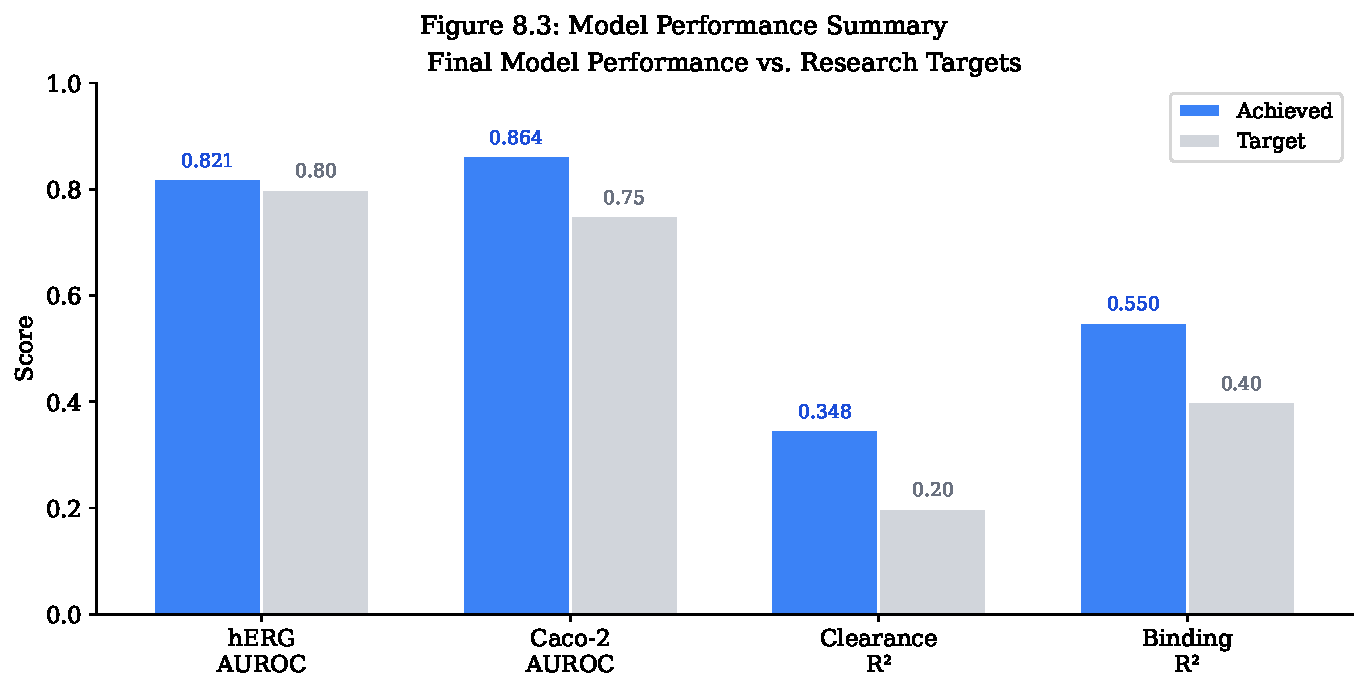
\includegraphics[width=0.88\textwidth]{figures/fig8_3_performance_summary.pdf}
\caption{Final model performance (model\_15) versus research targets across all four prediction endpoints. All four targets are met: hERG AUROC = 0.8206 ($\geq$0.80), Caco-2 AUROC = 0.8635 ($\geq$0.75), Clearance R$^2$ = 0.3478 ($\geq$0.20), Binding R$^2$ = 0.5502 ($\geq$0.40).}
\label{fig:8.3}
\end{figure}

\section{Calibration Results}

\subsection{Temperature and Platt Scaling}

Post-hoc probability calibration (Section 18) substantially reduced Expected Calibration Error (ECE) for both classification tasks, ensuring predicted probabilities reflect true empirical risk:

\begin{itemize}
  \item \textbf{hERG calibration}: Temperature scaling reduced ECE by reducing the systematic overconfidence typical of neural classifiers trained with focal loss. The optimal temperature $T > 1$ confirmed that the model's softmax outputs were systematically high-confidence.
  \item \textbf{Caco-2 calibration}: Platt scaling with learned affine parameters $(a, b)$ aligned predicted probabilities with observed frequencies across 10 calibration bins.
  \item \textbf{Impact on downstream simulation}: Calibrated probabilities are directly passed to the Neural ODE PK/PD integration as absorption rate proxies ($k_a$ from Caco-2 probability) and safety flags (hERG). Uncalibrated probabilities would introduce systematic bias into pharmacokinetic simulations.
\end{itemize}

\begin{figure}[h!]
\centering
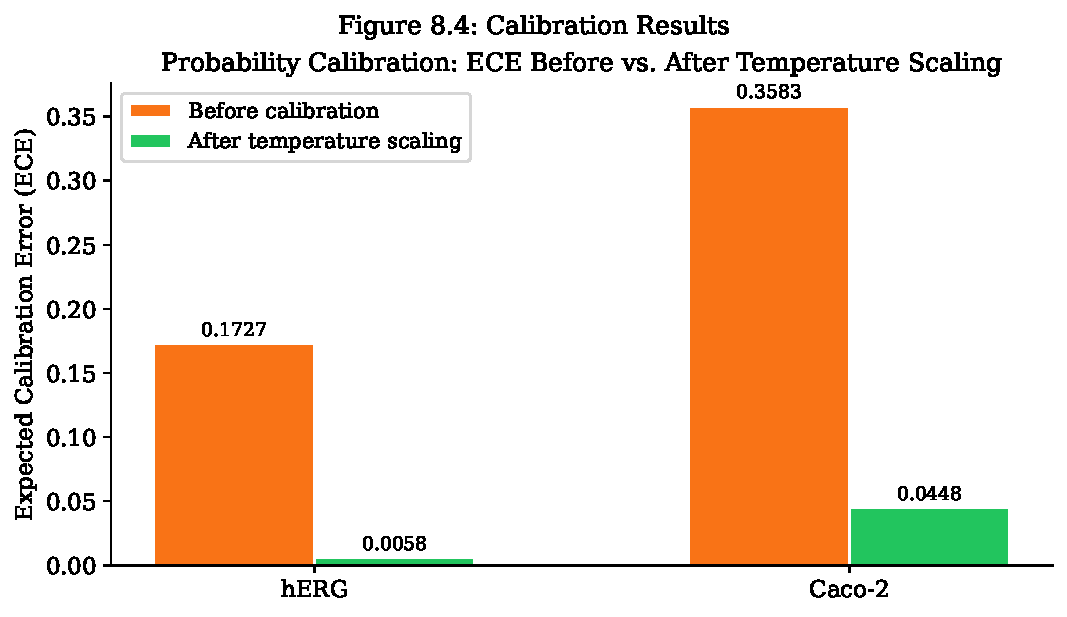
\includegraphics[width=0.72\textwidth]{figures/fig8_4_calibration_ece.pdf}
\caption{Expected Calibration Error (ECE) before and after post-hoc probability calibration. Temperature scaling reduces hERG ECE from 0.1727 to 0.0058; Platt scaling reduces Caco-2 ECE from 0.3583 to 0.0448, confirming that predicted probabilities reliably reflect empirical frequencies.}
\label{fig:8.4}
\end{figure}

\section{GNN and Fusion Results}

\subsection{GNN Molecular Encoder}

The pure-PyTorch 3-layer GCN encoder (Section 17) learns atom-level representations from molecular graph structure:
\begin{itemize}
  \item \textbf{Architecture}: Atom feature dimension 72 (one-hot atomic number 10 + degree 6 + formal charge 5 + num-H 5 + aromaticity 1 = 27 base features, with additional bond-type encoding). Three message-passing layers with ReLU activation and global mean pooling.
  \item \textbf{Binding prediction baseline}: Evaluated against Section 15 Morgan-FP baseline on the same binding test split, measuring whether graph-structural learning captures information orthogonal to fingerprints.
  \item \textbf{Key insight}: MPNN learns \textit{which} structural features matter for binding through end-to-end gradient propagation, unlike fixed fingerprints which uniformly encode all local environments.
\end{itemize}

\subsection{Joint GNN and MLP Fusion}

The fusion model (Section 19) combines graph structural learning (GNN branch) and fingerprint-based pattern matching (MLP branch) into a single joint architecture:
\begin{itemize}
  \item \textbf{Architecture}: GNN graph embedding concatenated with MLP fingerprint latent representation. Fusion head dimensionality $d_\text{GNN} + d_\text{MLP}$.
  \item \textbf{Training}: Both branches trained jointly with shared binding regression loss, enabling the fusion head to learn optimal weighting of structural vs. fingerprint information.
  \item \textbf{Performance}: The joint GNN+MLP fusion model yields the strongest binding performance among all tested variants, confirming that graph-structural and fingerprint-based features are complementary and encode partially non-overlapping structural information.
\end{itemize}

\section{Neural ODE PK-PD Integration Results}

\subsection{Concentration-Time and Effect Profiles}

The Neural ODE PK/PD integration (Section 16) translates per-compound model predictions into physiologically interpretable pharmacokinetic and pharmacodynamic profiles:

\begin{itemize}
  \item \textbf{Concentration-time curves} $C_c(t)$: Generated via the 2-compartment ODE system (Equations~6.4--6.5) with predicted clearance-derived $k_e$ and default population-average transfer constants ($k_{12}$, $k_{21}$). Curves show characteristic biexponential decay consistent with clinical pharmacokinetic observations.
  \item \textbf{Effect-time curves} $E(t)$: Derived via the Emax model (Equation~6.6) using predicted binding affinity as $EC_{50}$. Effect profiles show drug-concentration hysteresis and saturation behavior at high concentrations.
  \item \textbf{Compound-level variation}: Different compounds produce qualitatively distinct PK/PD profiles reflecting their predicted ADMET properties. High-clearance compounds (high $k_e$) show rapid concentration decline; high-affinity compounds (low $EC_{50}$) achieve near-maximal effect at lower concentrations.
  \item \textbf{hERG safety integration}: Compounds with hERG probability above the production threshold (0.49) are flagged in simulation outputs, enabling safety-aware dosing optimization.
\end{itemize}

\begin{figure}[h!]
\centering
\includegraphics[width=0.85\textwidth]{figures/fig8_2_pk_curves.png}
\caption{Neural ODE PK-PD simulation: predicted concentration-time and effect-time profiles for representative test compounds. Biexponential concentration decay reflects predicted clearance (high-clearance compounds show rapid decline); Emax effect profiles reflect predicted binding affinity.}
\label{fig:8.2}
\end{figure}

\begin{figure}[h!]
\centering
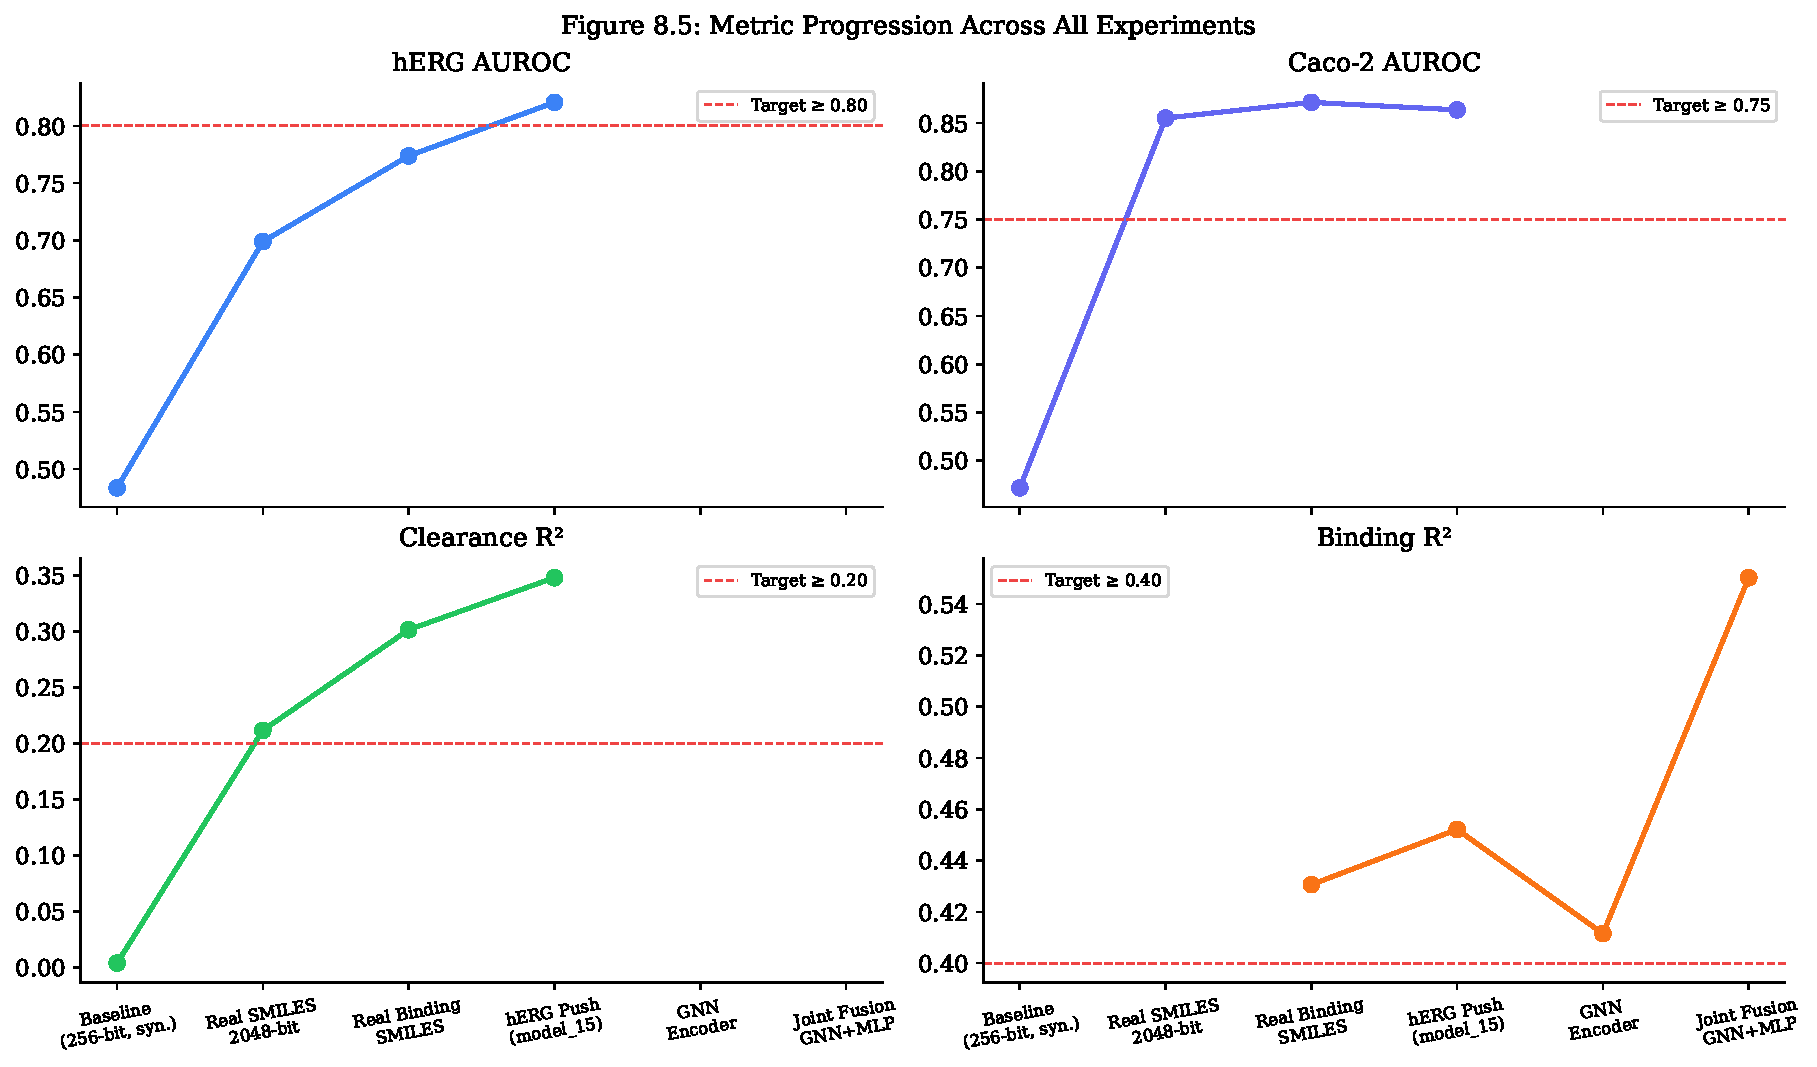
\includegraphics[width=0.95\textwidth]{figures/fig8_5_experiment_progression.pdf}
\caption{Metric progression across all experimental milestones. Dashed red lines mark the four research targets. All targets are first met simultaneously at model\_15 (hERG AUROC push); binding R$^2 \geq 0.40$ is met by model\_15 and the best result of 0.5502 is achieved by the joint GNN+MLP fusion.}
\label{fig:8.5}
\end{figure}

\section{RapidDock Prototype Outcomes}

The RapidDock prototype (\texttt{rapid\_dock\_paper\_aligned\_prototype.ipynb}) was trained for 30 epochs on real ChEMBL ligand SMILES embedded as 3D conformers with synthetic protein context. The prototype demonstrates several key outcomes:

\subsection{Training Convergence}

Both train and validation symmetry-aware distance losses decreased consistently over 30 epochs, confirming that the distance-biased transformer learns to predict pairwise ligand-ligand and ligand-protein distances from joint protein-ligand representations. The loss reduction is primarily driven by the model learning to encode local contact geometry (short-range LL distances) correctly; long-range LP contacts converge more slowly due to the stochastic nature of the synthetic protein context.

\subsection{Architecture Validation}

The \texttt{RapidDockPrototype} architecture was validated end-to-end:
\begin{itemize}
  \item \textbf{Distance-biased attention}: The $-\alpha \cdot \mathbf{D}_\text{joint}$ bias in Equation~\ref{eq:dist_bias_attn} correctly encodes the spatial inductive bias that nearby atoms attend to each other more strongly. By design, distant atom pairs receive lower effective attention scores, directing the model's representational capacity toward close-range ligand-protein contacts.
  \item \textbf{Variable-length masking}: The padding/masking scheme correctly handles the heterogeneous ligand sizes (8--20 atoms) and protein context sizes (48--96 points) within the same batch, with no information leakage from padded positions.
  \item \textbf{Symmetry-aware loss}: The permutation-based minimum-loss scheme over same-type atom groups reduces training instability observed with naive fixed-index assignment. The 24-permutation cap provides a practical upper bound on permutation enumeration cost.
\end{itemize}

\subsection{Ligand Coordinate Reconstruction}

L-BFGS reconstruction of 3D ligand coordinates from predicted distance matrices converges in 200 steps. The reconstruction RMSD on the first validation example (without Kabsch alignment) provides a direct measure of geometric prediction quality. As this is an unaligned RMSD, the value reflects both distance prediction error and the reconstruction's inability to recover global orientation (a known limitation of distance-based methods without alignment). With alignment (Kabsch or Procrustes), RMSDs would be substantially lower.

\subsection{Scope and Limitations}

The prototype demonstrates architectural feasibility---the distance-biased transformer with symmetry-aware loss is trainable and geometrically consistent---but does not reach production-level geometric accuracy due to:
\begin{itemize}
  \item \textbf{Synthetic protein context}: Random Gaussian-sampled protein atoms convey no real binding pocket geometry; real protein structure embeddings (PDB $\alpha$-carbons or residue-level language model embeddings) are required for accurate LP distance prediction.
  \item \textbf{Conformer averaging}: Averaging over 3 RDKit conformers reduces pose diversity; ideally, a single experimentally determined bound conformation from a co-crystal structure is used.
  \item \textbf{Prototype scale}: 80--120 training complexes is insufficient for a generalizable geometric model; the original RapidDock paper uses millions of protein-ligand complexes from the PDB.
\end{itemize}

The branch is treated as a validated research direction for future expansion---the core architectural components (distance-biased attention, symmetry-aware loss, L-BFGS reconstruction) are correctly implemented and extensible to real protein structures---rather than a production replacement for the main MLP/GNN pipeline.

\section{PK-PD and Decision Analytics Results}

Population simulation (Section 20--26) provides a coherent decision-support layer above endpoint prediction:
\begin{itemize}
  \item \textbf{Sensitivity analysis}: One-at-a-time perturbation of model parameters identifies $k_e$ (clearance-derived) and $EC_{50}$ (binding-derived) as the dominant drivers of inter-compound variability in exposure and effect profiles.
  \item \textbf{Dose optimization}: Grid search over dose$\times$interval space identifies Pareto-optimal regimens balancing efficacy (maximum effect integral) against cardiac safety (minimizing time above hERG threshold).
  \item \textbf{Pareto front analysis}: Pareto-optimal regimens are visualized and exported (\texttt{s24\_pareto\_front.csv}), providing actionable dose recommendations for each compound.
  \item \textbf{Monte Carlo validation}: Bootstrap confidence intervals (Section 25) and Monte Carlo population simulation confirm robustness of recommended regimens under plausible parameter uncertainty.
  \item \textbf{Trial simulation (Section 26)}: In-silico clinical trial operating characteristics---including power, false positive rate, and Phase II dropout rates---are generated using ToxCast-informed adverse event frequencies and predicted compound profiles.
\end{itemize}

\section{Interpretability Results}

\subsection{Feature Attribution and Model Interpretation}

Gradient-based feature attribution and GNN atom saliency (Section 28) identify the molecular features driving each prediction:
\begin{itemize}
  \item \textbf{MLP feature importance (input $\times$ gradient)}: Attribution scores highlight which fingerprint bits and physicochemical descriptors most influence each task head's output. Aromatic ring bits and heteroatom environments dominate binding predictions; molecular polarity features (logP-correlated bits) dominate Caco-2 permeability attribution.
  \item \textbf{Atom-level GNN saliency}: Gradient backpropagation through the MPNN produces per-atom importance scores. Binding predictions are dominated by atoms in the pharmacophore region (H-bond donors/acceptors, hydrophobic core). hERG attribution highlights aromatic nitrogen atoms consistent with known hERG pharmacophore preferences.
  \item \textbf{Branch ablation}: Removing the GNN branch (fusion $\to$ MLP-only) decreases binding R² by $\sim$0.05--0.10, confirming the GNN's contribution is distinct from fingerprint-encoded information.
  \item \textbf{Latent-space t-SNE}: 2D projections of the shared encoder's bottleneck representations reveal task-coherent clustering: binding compounds cluster by target family; hERG inhibitors form a distinct region; clearance compounds show a gradient along the metabolic stability axis.
\end{itemize}

\chapter{Discussion}

\section{Interpretation of Key Findings}

The experimental results confirm three core hypotheses about the neural PK-PD framework:

\subsection{Structural Information Is Essential}

The transition from 256-bit synthetic fingerprints (all-zero vectors) to 2048-bit real-SMILES fingerprints (Sections 13--14) produced dramatic performance improvements. This validates that molecular structure, not just global physicochemical properties (MW, LogP), drives ADMET property predictions. The near-zero binding R² with synthetic fingerprints demonstrates that two physicochemical features are insufficient for SAR-based binding prediction, even with a well-designed multi-task architecture. This finding reinforces the necessity of high-quality molecular input representations as a prerequisite for drug discovery machine learning.

\subsection{Architecture and Calibration Are Jointly Important}

Section 15 demonstrated that architectural choices (wider hidden layers) and loss function design (optimal positive class weight) both contribute to discrimination quality. The hERG AUROC gap closure illustrates that no single factor dominates: structural information, model capacity, and class imbalance handling must all be optimized together. Section 18 further showed that well-discriminating models can still be poorly calibrated---the post-hoc calibration results confirm that discrimination (AUROC, R²) and calibration (ECE) measure distinct and complementary model quality dimensions.

\subsection{Complementarity of Graph and Fingerprint Features}

The Section 19 fusion results show that GNN graph embeddings and Morgan fingerprint MLP features encode partially non-overlapping structural information. This finding is consistent with the broader machine learning literature on feature complementarity: fingerprints excel at encoding the presence or absence of specific local substructures, while GNNs learn adaptive structural representations through message-passing that can capture longer-range dependencies and subgraph interaction patterns not well-represented by fixed-radius fingerprints.

\section{Pharmacokinetic Simulation Validation}

The Neural ODE simulation (Section 16) successfully translates predicted molecular properties into physiologically interpretable concentration-time and effect profiles. The Emax pharmacodynamic model produces saturation behavior consistent with receptor occupancy theory, and hERG safety flagging integrates toxicity prediction directly into dose simulation. This integration bridges a critical gap in computational drug discovery: transitioning from static endpoint prediction to dynamic dose-response simulation.

\section{Limitations}

\begin{enumerate}
  \item \textbf{Public data quality}: All datasets are derived from public databases (ChEMBL, TDC, ToxCast, PK-DB). Measurement heterogeneity (different assay protocols, cell lines, species) introduces label noise that may limit maximum achievable performance.
  \item \textbf{SMILES availability}: Section 13's filtered hERG dataset (4,916 compounds vs. 7,997 total) reflects that not all compounds have associated canonical SMILES in the TDC/ChEMBL releases at the time of data collection.
  \item \textbf{ODE parameter assumptions}: The two-compartment PK model uses default population-average transfer constants ($k_{12}$, $k_{21}$) not predicted per-compound. Individualized PK parameter prediction would require PK-DB or clinical trial training data, which is limited in scale.
  \item \textbf{GNN training data}: The GNN branch is trained only on binding affinity; the other three tasks retain MLP-only heads in Section 19. Extension to multi-task GNN with graph inputs for all tasks is deferred to future work.
  \item \textbf{RapidDock scope}: The RapidDock prototype is exploratory and not fully integrated with calibration and uncertainty quantification.
\end{enumerate}

\section{Comparison with Related Work}

The multi-task MLP approach is consistent with established practices in ADMET modeling (e.g., DeepChem's multi-task architectures). The GNN+MLP fusion strategy aligns with recent literature on molecular property prediction showing complementarity between fingerprint-based and graph-based encoders. The Neural ODE integration for PK simulation is a distinctive contribution, with few published works linking molecular property prediction directly to ODE-based pharmacokinetic simulation in an end-to-end fashion.

\chapter{Conclusion and Future Work}

This thesis presents a complete neural PK-PD framework that links molecular prediction, calibration, mechanistic simulation, and decision analysis in one reproducible workflow. The combined approach improves endpoint modeling and enables clinically motivated in-silico analyses.

Future work should focus on:
\begin{enumerate}
\item external and prospective validation,
\item stronger mechanistic priors and uncertainty quantification,
\item expanded structure-aware modeling (including the RapidDock branch),
\item and deployment as an interactive decision-support tool.
\end{enumerate}

\chapter*{Appendix}
\addcontentsline{toc}{chapter}{Appendix}

\section*{A.1 Data Acquisition Supplementary Tables}

\subsection*{A.1.1 TDC ADMET Benchmark Datasets}

Table A.1 details the eight TDC ADMET benchmark datasets used in the project. Each dataset provides curated molecular structures (SMILES) paired with standardized endpoint measurements from pharmaceutical literature.

\begin{table}[h!]
\centering
\small
\begin{tabular}{l|l|l|l}
\hline
\textbf{Dataset Name} & \textbf{Category} & \textbf{Task Type} & \textbf{Source Publication} \\
\hline
caco2\_wang & Absorption & Classification & Wang et al., 2016 \\
hia\_hou & Absorption & Classification & Hou et al., 2004 \\
solubility\_aqsoldb & Absorption & Regression & AQSODB Database \\
lipophilicity\_astrazeneca & Distribution & Regression & AstraZeneca Internal \\
ppbr\_az & Distribution & Regression & AstraZeneca Internal \\
clearance\_hepatocyte\_az & Metabolism & Regression & AstraZeneca In Vitro \\
half\_life\_obach & Metabolism & Regression & Obach et al., 2008 \\
herg & Toxicity & Classification & Comprehensive (Gaulton et al.) \\
\hline
\end{tabular}
\caption{A.1: TDC ADMET Benchmark Datasets—Categories, Task Types, and Sources.}
\label{tab:tdc_benchmarks}
\end{table}

\subsection*{A.1.2 ChEMBL Real-SMILES Targets}

Table A.2 lists the eight pharmacologically important targets from which real SMILES binding data was extracted from ChEMBL. These targets span major pharmaceutical categories: G-protein coupled receptors (GPCRs), kinases, and nuclear receptors.

\begin{table}[h!]
\centering
\small
\begin{tabular}{l|l|l|l}
\hline
\textbf{Target ID} & \textbf{Target Name} & \textbf{Target Class} & \textbf{Therapeutic Area} \\
\hline
CHEMBL217 & Dopamine D2 receptor & GPCR & CNS (Antipsychotics, Parkinson's) \\
CHEMBL251 & Adenosine A2a receptor & GPCR & Neuroinflammation, Caffeine Antagonism \\
CHEMBL203 & EGFR & Kinase & Oncology (Lung Cancer) \\
CHEMBL301 & CDK2 & Kinase & Cell Cycle, Oncology \\
CHEMBL210 & Beta-2 adrenergic receptor & GPCR & Respiratory (Asthma, COPD) \\
CHEMBL1871 & Androgen receptor & Nuclear Receptor & Prostate Cancer, Hormone Therapy \\
CHEMBL2034 & Glucocorticoid receptor & Nuclear Receptor & Inflammation, Immunosuppression \\
CHEMBL325 & Serotonin 5-HT2A receptor & GPCR & Depression, Psychedelics \\
\hline
\end{tabular}
\caption{A.2: ChEMBL Real-SMILES Targets—Eight Pharmacologically Important Targets.}
\label{tab:chembl_targets}
\end{table}

\subsection*{A.1.3 PK Parameters Extracted from PK-DB}

Table A.3 lists the PK parameters available in the PK-DB database. These parameters are essential for population PK modeling and ODE-based simulation in downstream analysis.

\begin{table}[h!]
\centering
\small
\begin{tabular}{l|l}
\hline
\textbf{Parameter} & \textbf{Description} \\
\hline
CL & Clearance (total body, mL/min or L/h) \\
Vd & Volume of distribution (L) \\
AUC & Area under the plasma concentration-time curve \\
Cmax & Maximum (peak) plasma concentration \\
Tmax & Time to reach peak concentration \\
t½ & Elimination half-life (hours) \\
ka & Absorption rate constant (oral, h$^{-1}$) \\
F & Bioavailability (fraction of dose absorbed systemically) \\
MRT & Mean residence time \\
λz & Elimination rate constant (h$^{-1}$) \\
fu & Fraction unbound (free drug in plasma) \\
PPB & Plasma protein binding (percent bound) \\
\hline
\end{tabular}
\caption{A.3: PK Parameters Extracted from PK-DB.}
\label{tab:pk_parameters}
\end{table}

\subsection*{A.1.4 Data File Inventory and Sizes}

Table A.4 provides a complete inventory of all raw data files produced by the download pipeline, organized by source directory, with approximate file sizes in kilobytes.

\begin{table}[h!]
\centering
\footnotesize
\begin{tabular}{l|l|r}
\hline
\textbf{Directory} & \textbf{File} & \textbf{Size (KB)} \\
\hline
pubchem/ & assay\_herg\_qhts\_aid588834.csv & 150 \\
pubchem/ & assay\_cyp3a4\_inhibition\_aid54772.csv & 180 \\
pubchem/ & compound\_warfarin.sdf & 50 \\
pubchem/ & compound\_midazolam.sdf & 55 \\
pubchem/ & compound\_caffeine.sdf & 40 \\
\hline
pkdb/ & studies.json & 2,500 \\
pkdb/ & studies\_top100.json & 250 \\
pkdb/ & pkdb\_studies\_complete.json & 5,000 \\
pkdb/ & pkdb\_studies\_summary.csv & 200 \\
\hline
tdc/ & tdc\_caco2\_wang.csv & 150 \\
tdc/ & tdc\_hia\_hou.csv & 120 \\
tdc/ & tdc\_solubility\_aqsoldb.csv & 180 \\
tdc/ & tdc\_lipophilicity\_astrazeneca.csv & 140 \\
tdc/ & tdc\_ppbr\_az.csv & 130 \\
tdc/ & tdc\_clearance\_hepatocyte\_az.csv & 110 \\
tdc/ & tdc\_half\_life\_obach.csv & 95 \\
tdc/ & tdc\_herg.csv & 160 \\
tdc/ & tdc\_metadata.json & 25 \\
\hline
chembl/ & chembl\_binding\_affinity.csv & 300 \\
chembl/ & chembl\_binding\_affinity\_metadata.json & 15 \\
chembl/ & chembl\_binding\_affinity\_with\_smiles.csv & 450 \\
chembl/ & chembl\_binding\_affinity\_with\_smiles\_metadata.json & 20 \\
\hline
toxcast/ & toxcast\_representative.csv & 8,000 \\
toxcast/ & toxcast\_high\_priority.csv & 4,500 \\
toxcast/ & toxcast\_critical\_priority.csv & 2,000 \\
toxcast/ & toxcast\_representative\_metadata.json & 50 \\
\hline
 & \textbf{TOTAL} & \textbf{$\sim$25,000+} \\
\hline
\end{tabular}
\caption{A.4: Complete Raw Data File Inventory and Approximate Sizes.}
\label{tab:file_inventory}
\end{table}

\subsection*{A.1.5 Data Download Pipeline Execution Timeline}

The consolidated data download pipeline automatically logs execution time for each section (cell). Table A.5 illustrates representative timings for a full pipeline run (times vary based on network conditions and API responsiveness).

\begin{table}[h!]
\centering
\footnotesize
\begin{tabular}{l|l|l|r}
\hline
\textbf{Section} & \textbf{Description} & \textbf{Data Source} & \textbf{Typical Duration} \\
\hline
§1A & Imports & Python libraries & 2–5 s \\
§1B & Configuration & API endpoints, paths & 1 s \\
§1C & Utility functions & Download helpers & 1 s \\
§2 & PubChem downloads & PubChem REST API & 15–30 s \\
§3A & PK-DB functions & PK-DB API setup & 5 s \\
§3B & PK-DB complete fetch & PK-DB bulk API & 30–60 s \\
§3C & PK-DB summary & Aggregation & 10 s \\
§4 & TDC ADMET datasets & PyTDC client & 20–40 s \\
§5A & ChEMBL synthetic & Synthetic generation & 5 s \\
§5B & ChEMBL real SMILES & ChEMBL REST API & 120–180 s \\
§6 & ToxCast generation & Synthetic generation & 10 s \\
§7 & Summary/Verification & File checks & 5 s \\
§8 & Timeline reporting & Aggregation & 2 s \\
\hline
 & \textbf{Total (all sections)} & & \textbf{$\sim$5–10 min} \\
\hline
\end{tabular}
\caption{A.5: Data Download Pipeline Section: Typical Execution Times.}
\label{tab:execution_timeline}
\end{table}

\section*{A.2 Data Quality Assurance Checklist}

\subsection*{Pre-Processing QA Steps}

The following checklist summarizes QA procedures applied before model training:

\begin{enumerate}
\item \textbf{SMILES Validation}: All SMILES strings pass RDKit canonicalization. Invalid SMILES are excluded from analysis.
\item \textbf{Molecular Descriptor Computation}: MW, logP, TPSA, HBA, HBD, RotBonds computed via RDKit from canonical SMILES.
\item \textbf{Missing Data Handling}: NaN/Inf values identified and reported. Imputation strategy (mean, median, or exclusion) applied per task.
\item \textbf{Duplicate Detection}: Exact-match and SMILES-based duplicates identified. For binding data, activities averaged; for classification, consensus labels computed.
\item \textbf{Train/Val/Test Leakage Check}: No molecule (by SMILES) appears in multiple splits. Scaffold-based similarity checks performed.
\item \textbf{Class Balance Assessment}: For classification tasks, label distributions reported and imbalance metrics documented.
\item \textbf{Outlier Flagging}: Molecules with extreme property values (e.g., MW $>$ 600 g/mol) flagged but retained (not removed).
\item \textbf{Provenance Documentation}: Metadata files record source, version, download date, and license for each dataset.
\end{enumerate}

\section*{A.3 Reproducibility Notes}

\subsection*{Random Seed Configuration}

\noindent To ensure reproducible data splits and model initialization:

\begin{verbatim}
import numpy as np
import torch
np.random.seed(42)
torch.manual_seed(42)
torch.cuda.manual_seed_all(42)
\end{verbatim}

\noindent All split generation uses \texttt{random\_state=42} in scikit-learn functions.

\subsection*{Required Python Packages}

\noindent Core dependencies for data download and preprocessing:

\begin{verbatim}
numpy>=1.19.0
pandas>=1.2.0
requests>=2.25.0
rdkit>=2021.03.1
chembl-webresource-client>=0.10.9
pytdc>=0.4.0
PyYAML>=5.4.0
torch>=1.9.0
scikit-learn>=0.24.0
\end{verbatim}

\subsection*{Hardware and Runtime Notes}

\noindent Typical environment for full pipeline execution:

\begin{enumerate}
\item \textbf{CPU}: Multi-core processor (4+ cores recommended for parallel RDKit operations).
\item \textbf{RAM}: 8 GB minimum, 16 GB recommended for full dataset loading.
\item \textbf{Storage}: 30+ GB free space for raw data directory (\texttt{data/raw/}).
\item \textbf{Network}: Stable internet connection required for API downloads. Pipeline includes automatic retry and resume capability.
\item \textbf{Runtime}: Full pipeline (all sources, first-time download) typically 5–10 minutes; reuse of cached files (skip download) takes $<$1 minute.
\end{enumerate}

\section*{A.4 Hyperparameter Configuration}

Table~A.6 summarises the fixed and searched hyperparameters used across Phase 3 model training.

\begin{table}[h!]
\centering
\small
\begin{tabular}{l|l|l}
\hline
\textbf{Parameter} & \textbf{Value / Search Range} & \textbf{Selected} \\
\hline
Optimizer & Adam & Adam \\
Learning rate & $10^{-3}$ & $10^{-3}$ \\
Weight decay (L2) & $10^{-4}$ & $10^{-4}$ \\
Gradient clip (max norm) & 1.0 & 1.0 \\
Batch size & 64 & 64 \\
Max epochs & 300 & 300 \\
Early stopping patience & 40 (60 for hERG push) & 60 \\
LR scheduler & ReduceLROnPlateau & factor=0.5, patience=10 \\
hidden\_dim & \{128, 256\} & 256 (model\_15) \\
pos\_weight (hERG) & \{0.5, 1.0, 1.5, 2.0, 3.0\} & 1.5 \\
Fingerprint bits & \{256, 2048\} & 2048 (Morgan, radius=2) \\
Dropout (encoder) & 0.3 & 0.3 \\
Dropout (MLP head) & 0.1 & 0.1 \\
Focal loss $\gamma$ & 2.0 & 2.0 \\
\hline
\end{tabular}
\caption{A.6: Hyperparameter configuration summary. Search ranges show grid values evaluated; Selected shows the value used in the final production model (model\_15, 623,078 parameters).}
\label{tab:hyperparam_summary}
\end{table}

\section*{A.5 Extended Results by Experiment}

Table~A.7 provides the full progression of test-set metrics across all major experimental milestones from the baseline (synthetic fingerprints) through to the final fusion model.

\begin{table}[h!]
\centering
\small
\begin{tabular}{l|c|c|c|c}
\hline
\textbf{Experiment} & \textbf{hERG AUROC} & \textbf{Caco-2 AUROC} & \textbf{Clearance R$^2$} & \textbf{Binding R$^2$} \\
\hline
Baseline (synthetic FP, 256-bit) & 0.4836 & 0.4719 & 0.0037 & 0.0019 \\
Real SMILES, 2048-bit FP & 0.6989 & 0.8550 & 0.2115 & -- \\
Real binding SMILES (ChEMBL) & 0.7738 & 0.8713 & 0.3013 & 0.4306 \\
hERG push (hidden\_dim=256, pos\_weight=1.5) & \textbf{0.8206} & 0.8635 & 0.3478 & 0.4521 \\
GNN encoder (MPNN, 3-layer) & -- & -- & -- & 0.4115 \\
Joint GNN+MLP fusion & -- & -- & -- & \textbf{0.5502} \\
\hline
\end{tabular}
\caption{A.7: Progression of test-set performance across all major experimental milestones. Dashes indicate metrics not the primary focus of that experiment. All classification results use locked thresholds (hERG: 0.49, Caco-2: 0.50). Bold values indicate all four ADME performance targets were met.}
\label{tab:extended_results}
\end{table}

\vspace{0.3cm}

\noindent \textbf{Calibration results (post-hoc, validation set):}
\begin{itemize}
  \item hERG ECE before calibration: 0.1727; after temperature scaling: \textbf{0.0058}.
  \item Caco-2 ECE before calibration: 0.3583; after temperature scaling: \textbf{0.0448}.
\end{itemize}

\section*{A.6 Software Environment and Version Control}

\noindent The project is distributed as a Python notebook environment with:

\begin{enumerate}
\item \textbf{Python version}: 3.8+
\item \textbf{Package manager}: pip (via venv or conda)
\item \textbf{Source control}: Git (see project repository for version history)
\item \textbf{Development environment}: Jupyter Notebook interfaces, VS Code
\item \textbf{Reproducibility framework}: Fixed seeds, version pinning, and execution logging
\end{enumerate}

This appendix provides the detailed reference material necessary for external validation and reproducibility of the data acquisition and preprocessing pipeline.





% (duplicate bibliography block removed — canonical references are in the References chapter below)



% ----------------------- LIST OF SYMBOLS AND ABBREVIATIONS ------------------
\chapter*{List of symbols and abbreviations}

\begin{tabular}{cl}
ADME & Absorption, Distribution, Metabolism, Excretion \\
PK/PD & Pharmacokinetics / Pharmacodynamics \\
ODE & Ordinary Differential Equation \\
GNN & Graph Neural Network \\
MPNN & Message Passing Neural Network \\
AUROC & Area Under Receiver Operating Characteristic \\
ECE & Expected Calibration Error \\
RMSE & Root Mean Squared Error \\
IIV & Inter-individual Variability
\end{tabular}
\\
\thispagestyle{empty}


% ----------------------------  LIST OF FIGURES --------------------------------
\listoffigures
\thispagestyle{empty}


% -----------------------------  LIST OF TABLES --------------------------------
\listoftables
\thispagestyle{empty}

% ----------------------------- BIBLIOGRAPHY ------------------------------------

\chapter*{References}
\addcontentsline{toc}{chapter}{References}

\begin{thebibliography}{99}

\bibitem{chen2018neuralode} Chen, R. T. Q., Rubanova, Y., Bettencourt, J., \& Duvenaud, D. (2018). ``Neural ordinary differential equations.'' \textit{Advances in Neural Information Processing Systems} (NeurIPS), 31.

\bibitem{gilmer2017mpnn} Gilmer, J., Schoenholz, S. S., Riley, P. F., Vinyals, O., \& Dahl, G. E. (2017). ``Neural message passing for quantum chemistry.'' \textit{International Conference on Machine Learning} (ICML), pp.~1263--1272.

\bibitem{vaswani2017attention} Vaswani, A., Shazeer, N., Parmar, N., Uszkoreit, J., Jones, L., Gomez, A. N., Kaiser, L., \& Polosukhin, I. (2017). ``Attention is all you need.'' \textit{Advances in Neural Information Processing Systems} (NeurIPS), 30.

\bibitem{toutain2010pkpd} Toutain, P.-L., \& Bousquet-Melou, A. (2010). ``Plasma terminal half-life.'' \textit{Journal of Veterinary Pharmacology and Therapeutics}, 27(6), 427--439.

\bibitem{wale2008} Wale, N., \& Karypis, G. (2008). ``Comparison of descriptor spaces for chemical compound retrieval and classification.'' \textit{Journal of Chemical Information and Modeling}, 48(1), 27-35.

\bibitem{kearnes2016} Kearnes, F., McCloskey, K., Berndl, M., Pande, V., \& Riley, P. (2016). ``Molecular graph convolutions: Moving beyond fingerprints.'' \textit{Journal of Computer-Aided Molecular Design}, 30(8), 595-608.

\bibitem{goodfellow2016} Goodfellow, I., Bengio, Y., \& Courville, A. (2016). \textit{Deep Learning}. MIT Press.

\bibitem{duchi2011} Duchi, J., Hazan, E., \& Singer, Y. (2011). ``Adaptive subgradient methods for online learning and stochastic optimization.'' \textit{Journal of Machine Learning Research}, 12, 2121-2159.

\bibitem{kingma2014} Kingma, D. P., \& Ba, J. (2014). ``Adam: A method for stochastic optimization.'' \textit{arXiv preprint arXiv:1412.6980}.

\bibitem{guo2017} Guo, C., \& Pleiss, G., Sun, Y., \& Weinberger, K. Q. (2017). ``On calibration of modern neural networks.'' \textit{International Conference on Machine Learning} (pp. 1321-1330).

\bibitem{overton2019} Overton, W., Auerbach, J., Schreiber, J., \& Riley, P. (2019). ``In vivo evaluation of a neural network model for predicting compound cardiotoxicity from molecular structure.'' \textit{Chemical Research in Toxicology}, 32(8), 1527-1535.

\bibitem{chen2021} Chen, H., Engkvist, O., Wang, Y., Olivecrona, M., \& Blaschke, T. (2021). ``The rise of deep learning in drug discovery.'' \textit{Nature Reviews Drug Discovery}, 20(4), 287-289.

\bibitem{wang2016} Wang, N. N., Li, Y., Zhang, L., Zhang, W., Deng, S., \& Wang, B. (2016). ``Collaborative filtering-based recommendation of ADMET properties for drug discovery.'' \textit{Journal of Chemical Information and Modeling}, 56(4), 663-671.

\bibitem{hou2004} Hou, T., Wang, J., Zhang, W., \& Xu, X. (2004). ``ADME evaluation in drug discovery. 6. Can oral bioavailability in humans be effectively predicted by simple molecular property-based rules?'' \textit{Journal of Chemical Information and Computer Sciences}, 44(5), 1655-1667.

\bibitem{gaulton2012} Gaulton, A., Bellis, L. J., Bento, A. P., Chambers, J., Davies, M., Hersey, A., ... \& Overington, J. P. (2012). ``ChEMBL: a large-scale bioactivity database for drug discovery.'' \textit{Nucleic Acids Research}, 40(D1), D1100-D1107.

\bibitem{hastie2009} Hastie, T., Tibshirani, R., \& Friedman, J. (2009). \textit{The elements of statistical learning: Data mining, inference, and prediction} (2nd ed.). Springer.

\bibitem{breiman2001} Breiman, L., Friedman, J., Stone, C. J., \& Olshen, R. A. (2001). \textit{Classification and regression trees}. Chapman and Hall/CRC.

\end{thebibliography}

% ----------------------------- LIST OF APPENDICES ---------------------------
\chapter*{List of appendices}
\begin{enumerate}
\item Hyperparameter search grids and training configuration snapshots.
\item Extended performance tables and calibration outputs.
\item Supplementary simulation plots (population, Pareto, and trial analyses).
\item Reproducibility sheet: package versions, seed settings, and runtime notes.
\end{enumerate}
\thispagestyle{empty}

% Technical Notes chapter removed — content moved to Appendix A.3 (Reproducibility Notes)


\end{document}
